\documentclass[10pt]{article}
\usepackage[french]{babel}
\usepackage[utf8]{inputenc}
\usepackage[T1]{fontenc}
\usepackage{amsmath}
\usepackage{amsfonts}
\usepackage{amssymb}
\usepackage[version=4]{mhchem}
\usepackage{stmaryrd}
\usepackage{graphicx}
\usepackage[export]{adjustbox}
\graphicspath{ {./images/} }
\usepackage{caption}

\title{Méthodes générales d'analyse Partie 2 }

\author{}
\date{}


\begin{document}
\maketitle
\captionsetup{singlelinecheck=false}
Circuits électriques

ELECOO53-2

Introduction

\section*{Au dernier cours, nous avons vu}
\begin{itemize}
  \item Comment généraliser les concepts appris jusqu'à présent en utilisant la théorie des graphes appliquée à la PLK pour obtenir la méthode des noeuds
  \item Comment généraliser le théorème de Norton à plus de $n-1$ accès, puis comment réduire ce modèle à $x<n-1$ accès
\end{itemize}

\section*{Qu'allons nous faire dans ce cours ?}
\begin{itemize}
  \item Apprendre une méthode duale à la méthode des noeuds : la méthode des mailles
  \item Généraliser le théorème de Thévenin pour des circuits à plusieurs accès
  \item utile lorsqu'on souhaite identifier les paramètres ou simplifier un modèle d'une partie d'un circuit "au milieu" d'autres parties.
  \item Voire comment implémenter une méthode sur ordinateur
\end{itemize}

Méthode des mailles

\section*{Rappel}
Maille (loop): sous-graphe connexe dont tous les noeuds sont de degré 2 (=cycle).\\
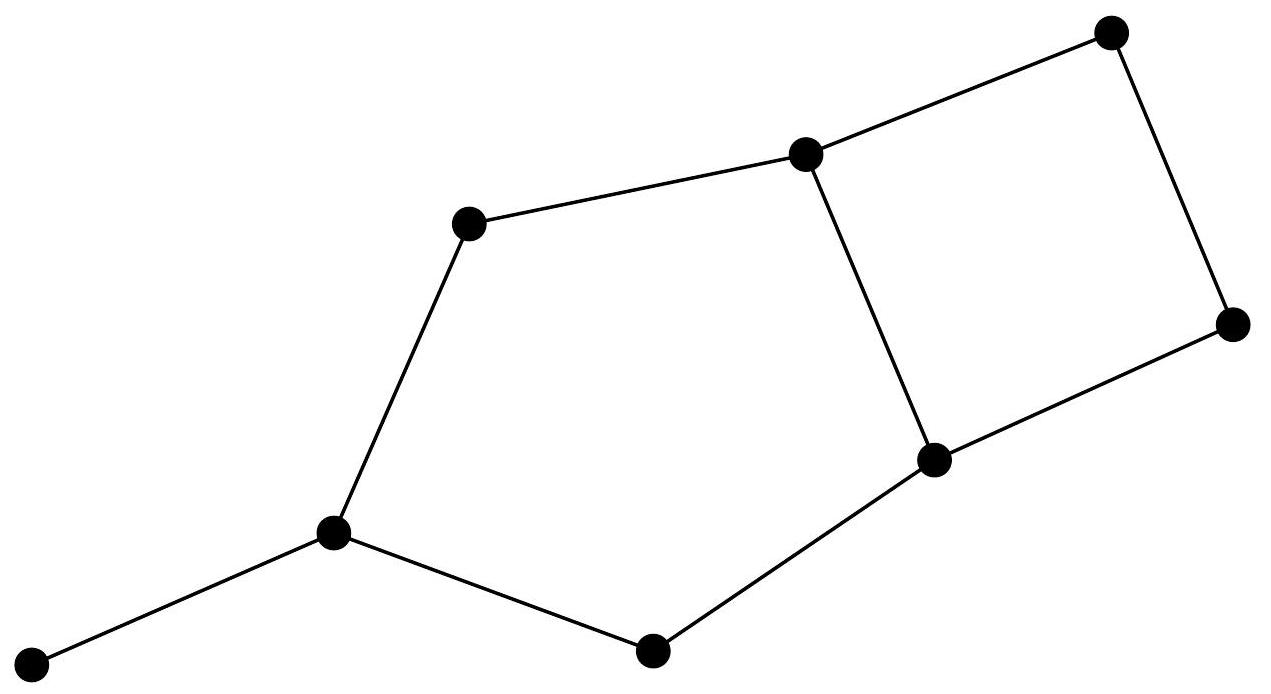
\includegraphics[max width=\textwidth, alt={}, center]{cbd435a9-cec2-4dd4-b13c-7b225dcc6548-06_694_1271_706_463}\\
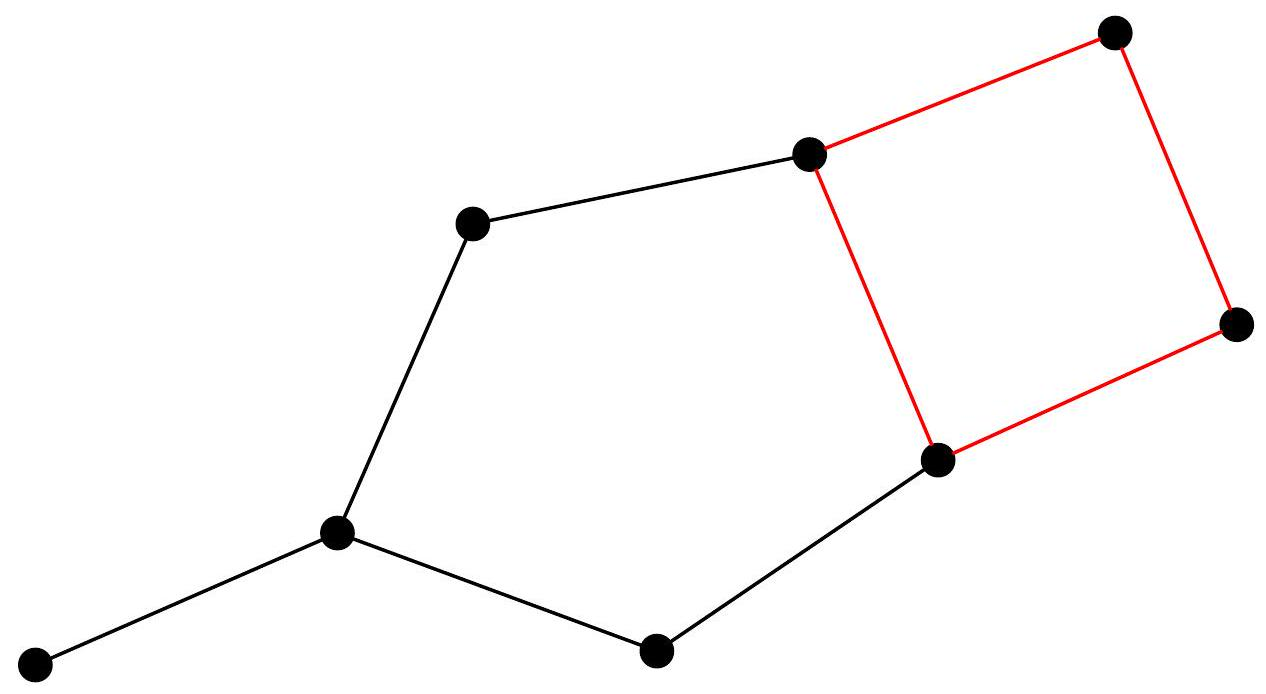
\includegraphics[max width=\textwidth, alt={}, center]{cbd435a9-cec2-4dd4-b13c-7b225dcc6548-06_694_1266_706_1824}\\
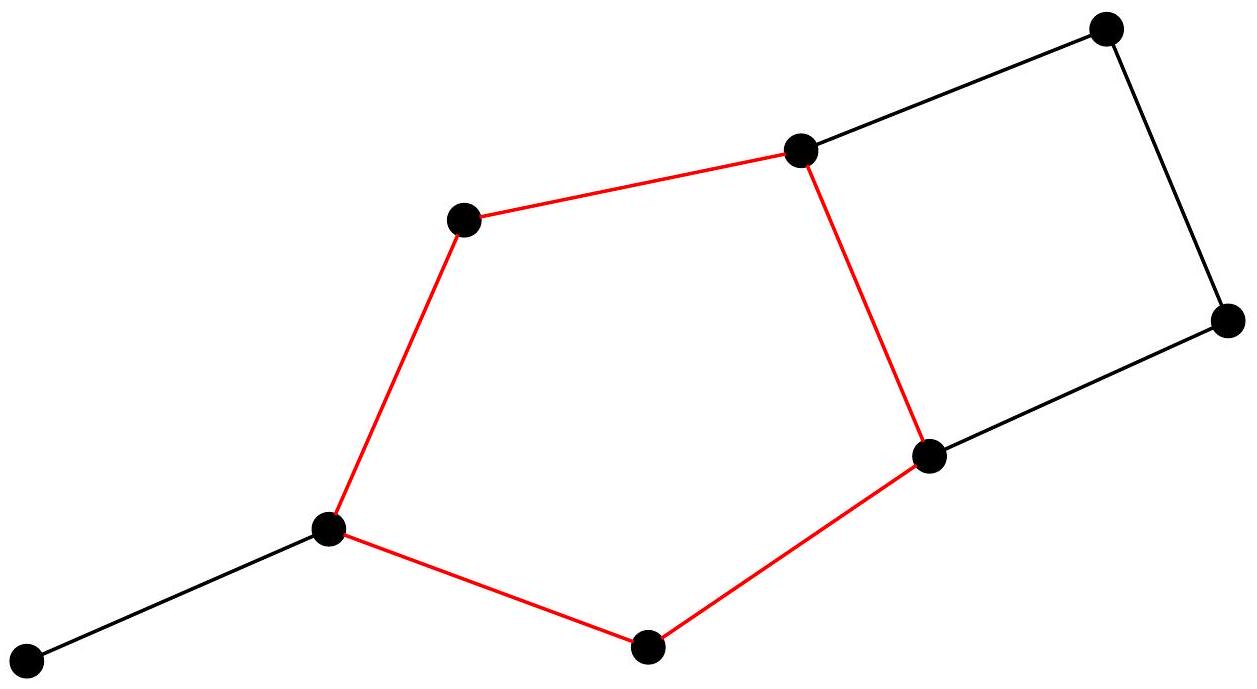
\includegraphics[max width=\textwidth, alt={}, center]{cbd435a9-cec2-4dd4-b13c-7b225dcc6548-06_689_1257_1623_468}\\
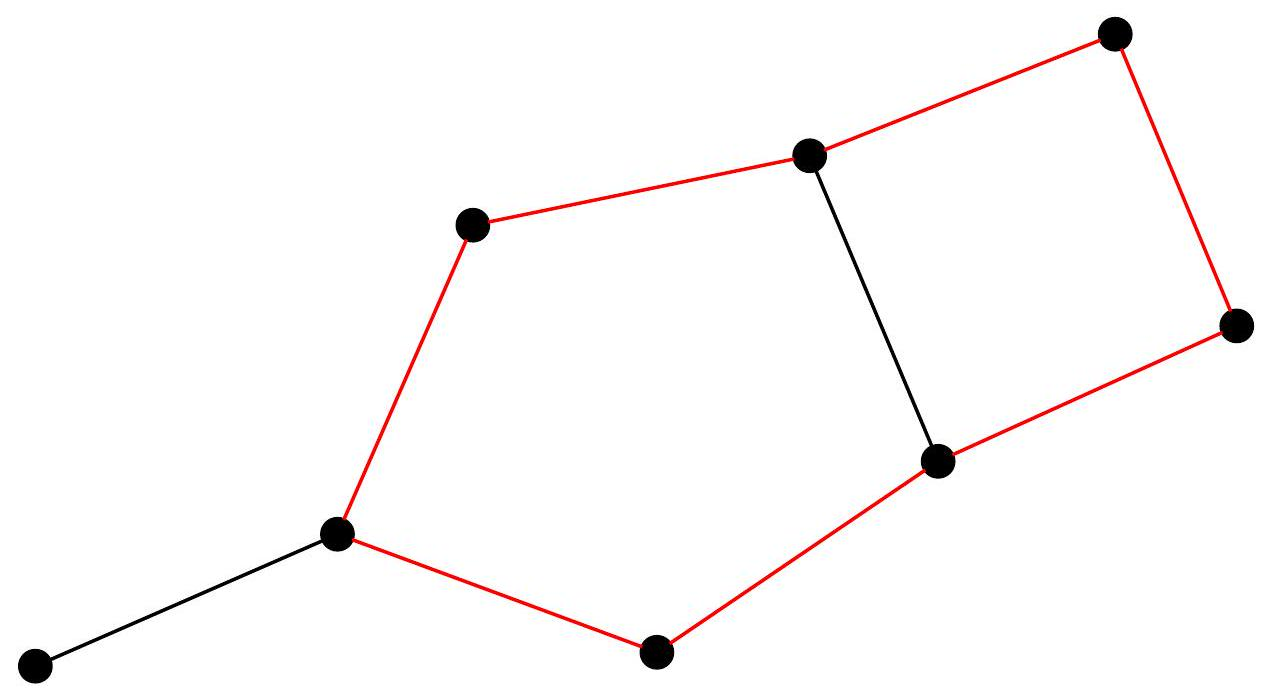
\includegraphics[max width=\textwidth, alt={}, center]{cbd435a9-cec2-4dd4-b13c-7b225dcc6548-06_694_1276_1618_1824}

\section*{Rappel}
Arbre : sous-graphe connexe qui contient tous les noeuds du graphe initial et qui ne comporte aucune maille. Branches restantes non incluses dans l'arbre $=$ maillons.

Nombre de branches de l'arbre pour réseau connexe : $n-1$\\
Nombre de maillons : $b-(n-1)$

\begin{figure}[h]
\begin{center}
  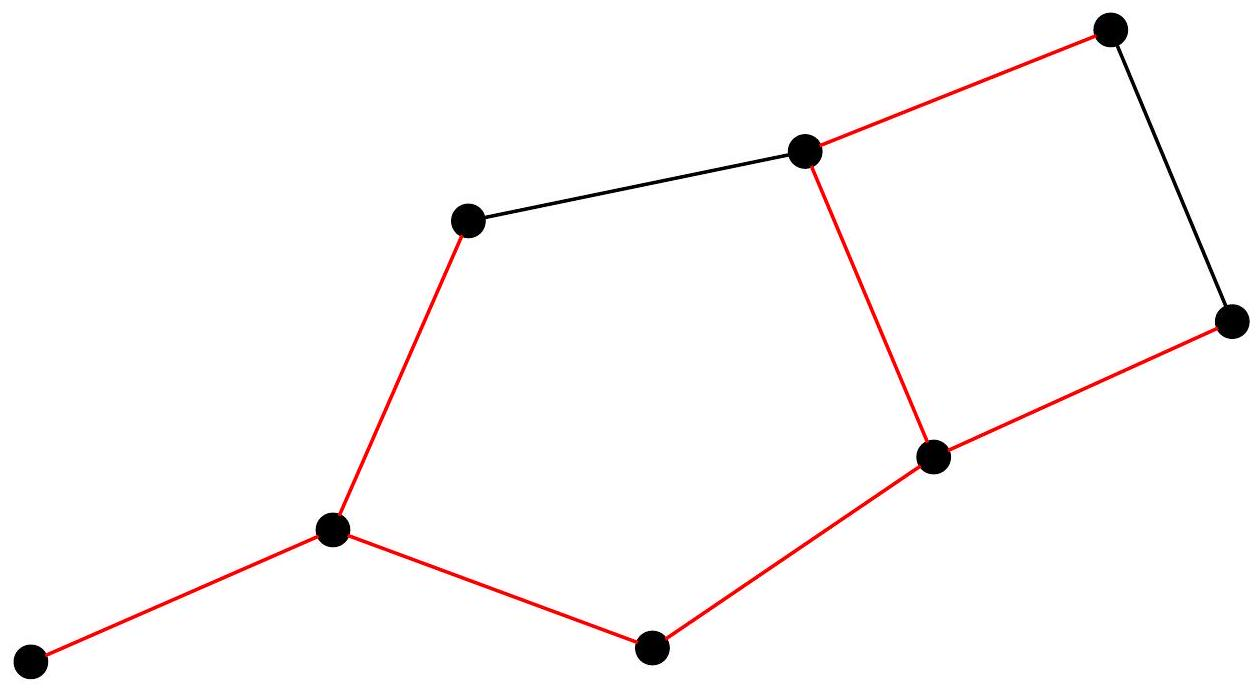
\includegraphics[alt={},max width=\textwidth]{cbd435a9-cec2-4dd4-b13c-7b225dcc6548-07_696_1260_1227_350}
\captionsetup{labelformat=empty}
\caption{\#branches: 7\\
\# maillons: 2}
\end{center}
\end{figure}

\section*{Rappel}
Maille fondamentale : pour un arbre donné, maille formée à partir d'un seul maillon et de branches de l'arbre\\
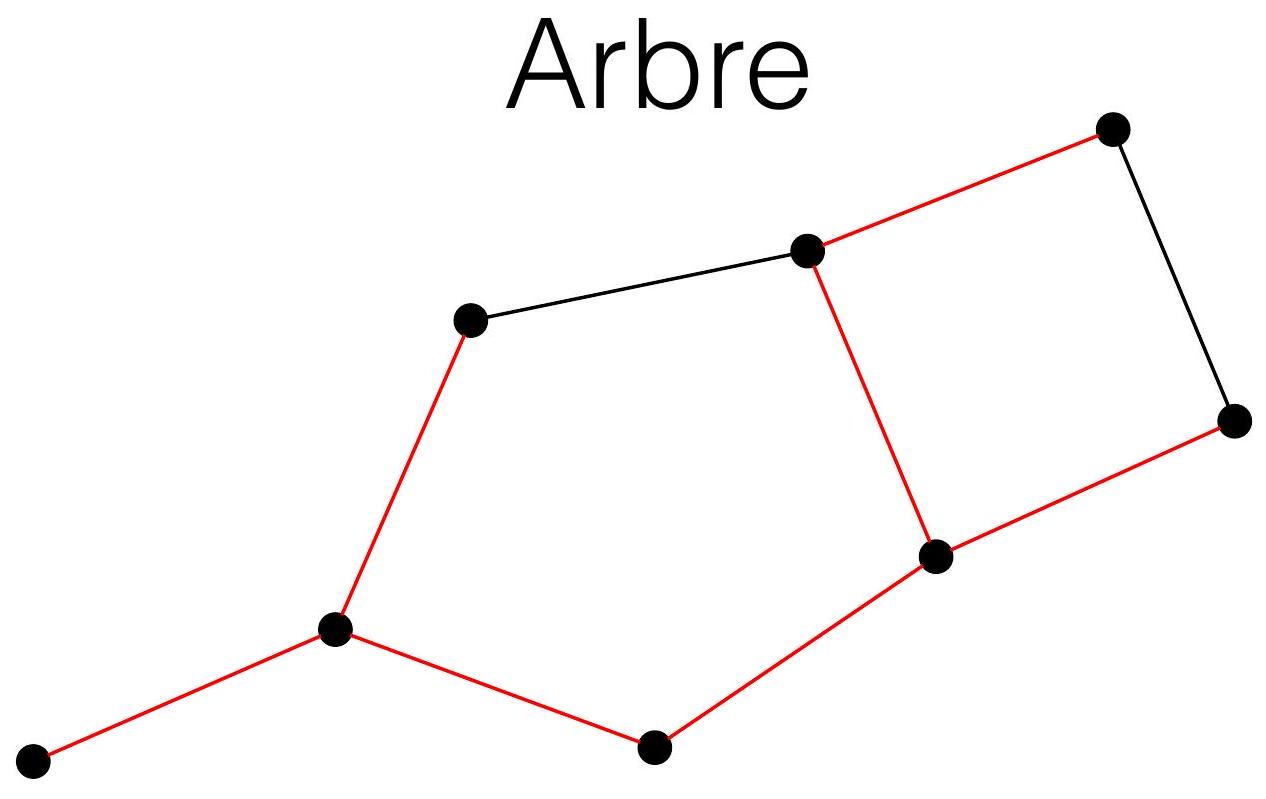
\includegraphics[max width=\textwidth, alt={}, center]{cbd435a9-cec2-4dd4-b13c-7b225dcc6548-08_799_1266_735_291}\\
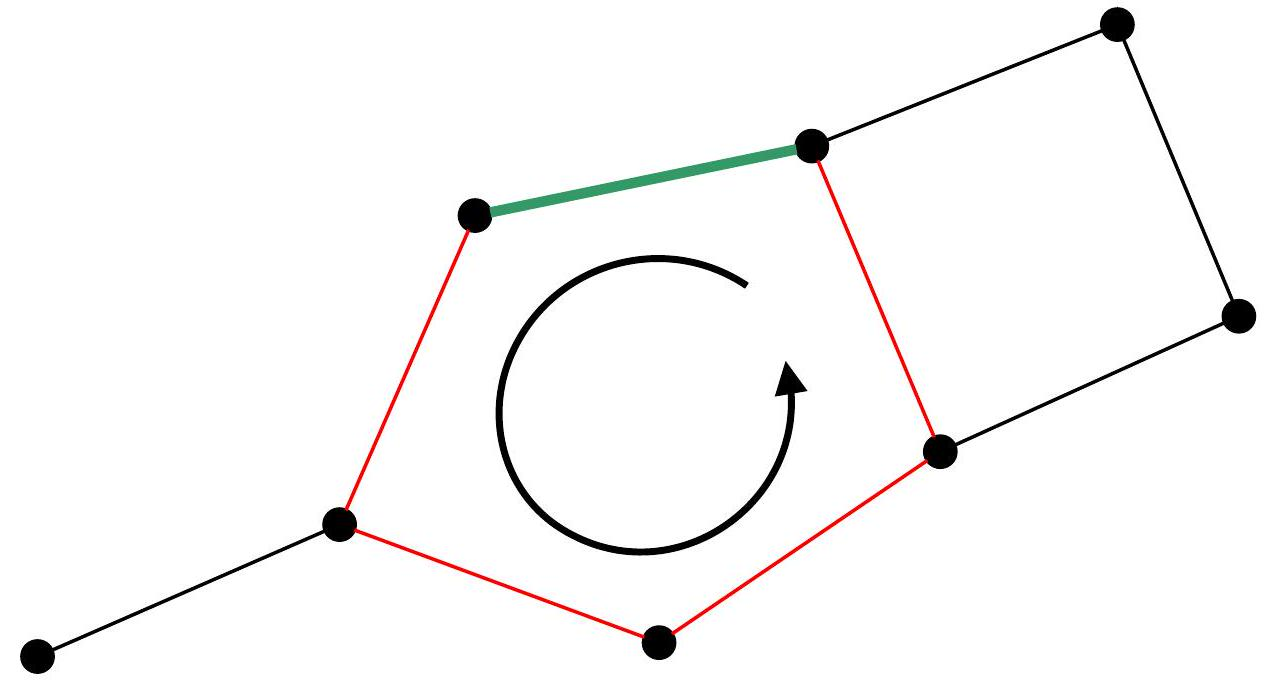
\includegraphics[max width=\textwidth, alt={}, center]{cbd435a9-cec2-4dd4-b13c-7b225dcc6548-08_684_1271_840_1700}\\
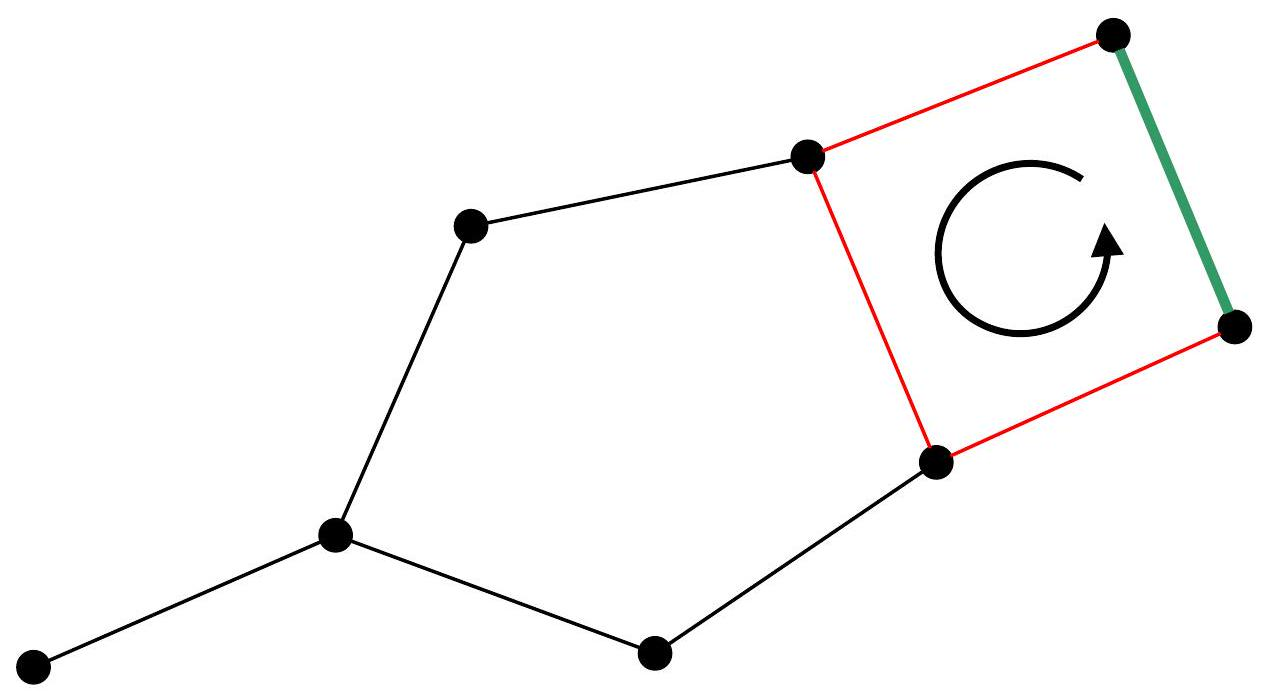
\includegraphics[max width=\textwidth, alt={}, center]{cbd435a9-cec2-4dd4-b13c-7b225dcc6548-08_693_1267_1614_1704}

\section*{Rappel}
\section*{2. Circuit et graphe}
On associe à un circuit un graphe orienté. L'orientation des branches est donnée par le sens du courant.

On se limite aux seuls graphes connexes.\\
On définit :

\begin{itemize}
  \item Etat électrique ou état : ( $\mathbf{u}_{B}(t), \mathbf{i}_{B}(t)$ ) ensemble des valeurs que prennent les courants et les tensions de branches à un instant donné
  \item $n$ : le nombre de noeuds du graphe ou du circuit
  \item $b$ : le nombre de branches
  \item le nombre de branches d'un arbre : $N=n-1$
  \item le nombre de mailles fondamentales : $M=b-(n-1)$
\end{itemize}

\section*{Rappel}
\begin{center}
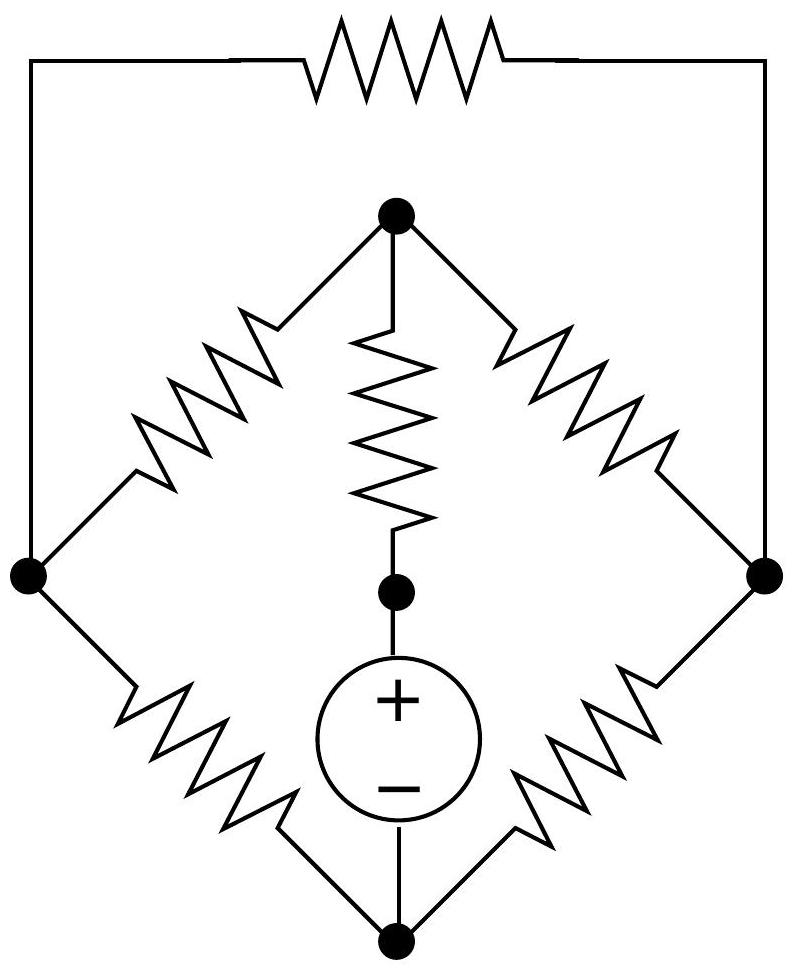
\includegraphics[max width=\textwidth, alt={}]{cbd435a9-cec2-4dd4-b13c-7b225dcc6548-10_975_799_315_558}
\end{center}

$$
n=5 \quad b=7 \quad N=4 \quad M=3
$$

\begin{figure}[h]
\begin{center}
  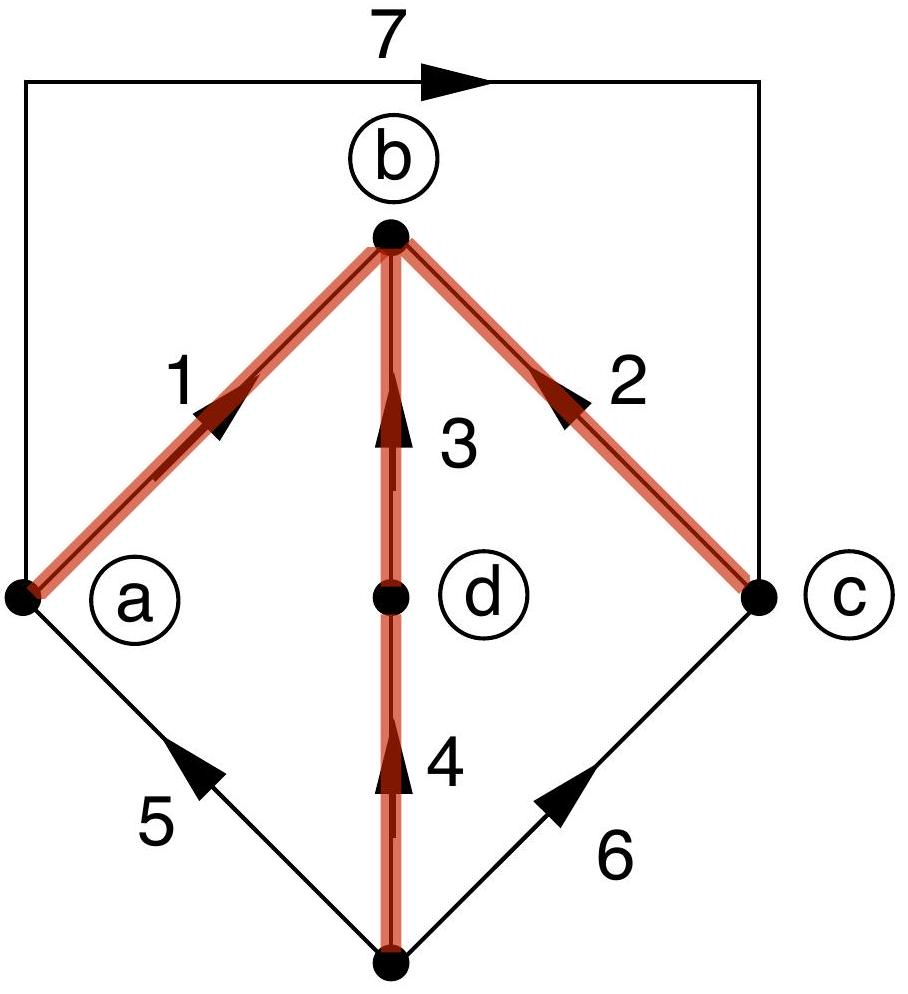
\includegraphics[alt={},max width=\textwidth]{cbd435a9-cec2-4dd4-b13c-7b225dcc6548-10_994_908_253_2001}
\captionsetup{labelformat=empty}
\caption{(e)}
\end{center}
\end{figure}

mailles : abdea , acea , acedba , . . . où face = abdea\\
arbre : branches $1,2,3,4$ mailles fondamentales : abdea, bcedb, bacb maillons correspondants : 5,6,7

\section*{Méthode des mailles}
Pour déterminer l'état électrique d'un système, la méthode des mailles consiste à résoudre le système linéaire suivant :

$$
\mathbf{R}_{\mathrm{M}} \mathbf{i}_{\mathrm{M}}=\mathbf{v}_{\mathrm{SM}}
$$

L'indice M signifie "Maille"\\
$\mathbf{i}_{\text {M }}$ est le vecteur des courants de maille

\begin{itemize}
  \item il contient les $b-n-1$ variables du système\\
$\mathbf{V}_{s}$ M est le vecteur des sources indépendantes de tension agissant dans les mailles
  \item déterminé par inspection, il caractérise l'impact des sources indépendantes de tension.
  \item Les tensions de branches en découlent, via la loi d'Ohm\\
$\mathbf{R}_{\mathrm{M} \text { est la matrice de résistances de mailles, }}$
  \item déterminée par inspection ou par expérimentation, elle caractérise le graphe du circuit passifié
\end{itemize}

\begin{figure}[h]
\begin{center}
\captionsetup{labelformat=empty}
\caption{1. Choisir un arbre et orienter les branches}
  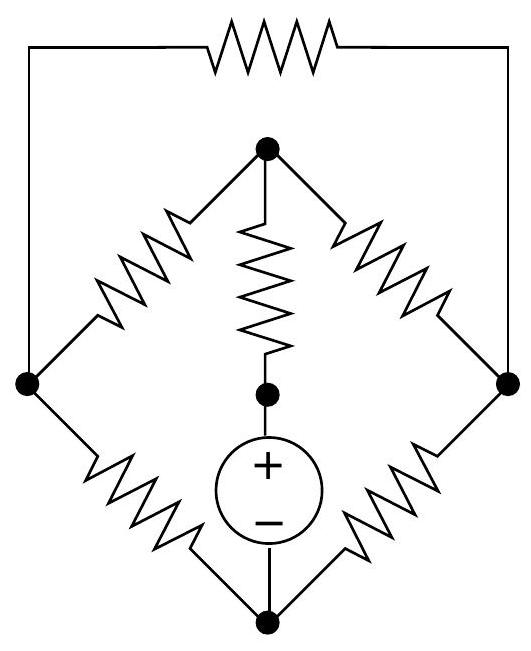
\includegraphics[alt={},max width=\textwidth]{cbd435a9-cec2-4dd4-b13c-7b225dcc6548-12_651_531_343_143}
\end{center}
\end{figure}

\begin{figure}[h]
\begin{center}
\captionsetup{labelformat=empty}
\caption{1. Choisir un arbre et orienter les branches}
  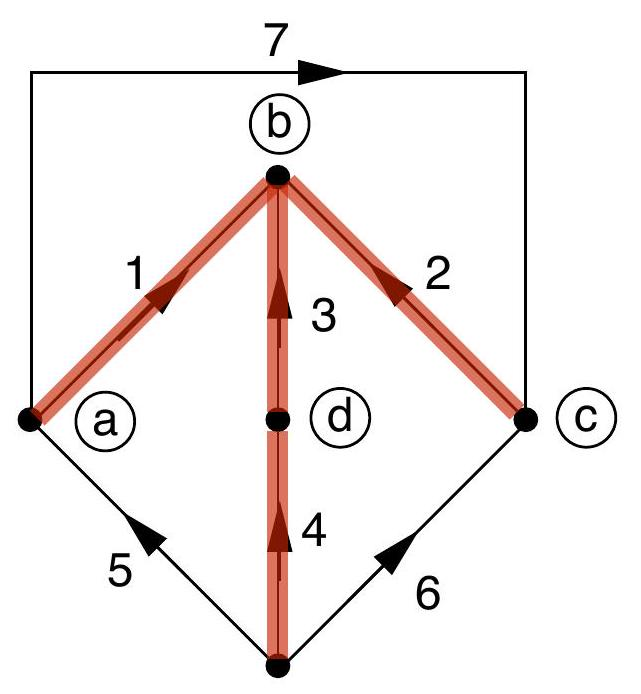
\includegraphics[alt={},max width=\textwidth]{cbd435a9-cec2-4dd4-b13c-7b225dcc6548-12_694_641_324_826}
\end{center}
\end{figure}

\begin{figure}[h]
\begin{center}
\captionsetup{labelformat=empty}
\caption{3. Déterminer $\mathbf{v}_{\mathrm{sM}}$}
  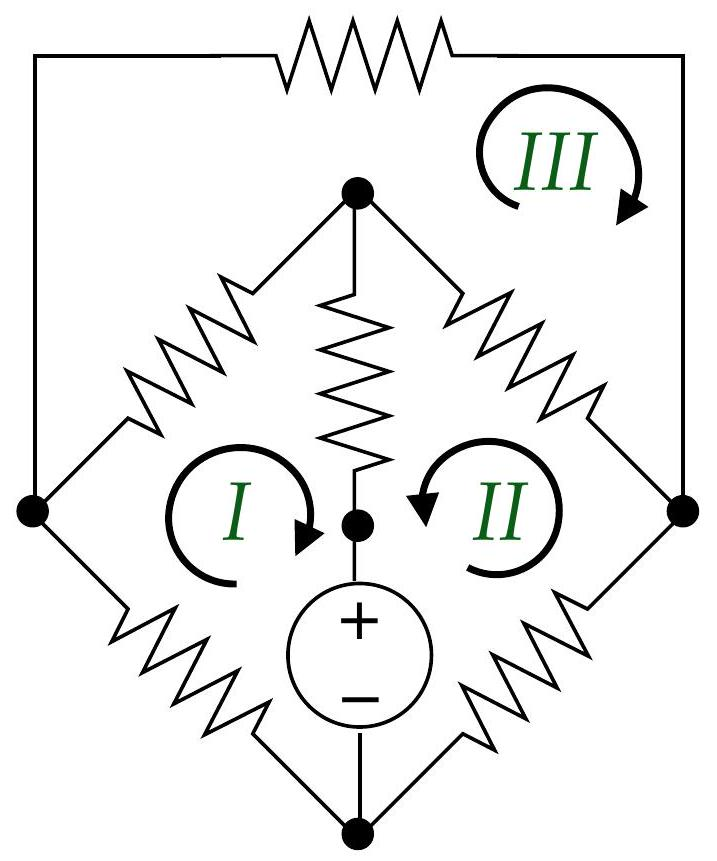
\includegraphics[alt={},max width=\textwidth]{cbd435a9-cec2-4dd4-b13c-7b225dcc6548-12_861_717_1384_396}
\end{center}
\end{figure}

$$
\mathbf{v}_{s \mathrm{M}}=(?, ?, ?)
$$

\begin{enumerate}
  \setcounter{enumi}{1}
  \item Déterminer $\mathbf{R}_{\mathrm{M}}$\\
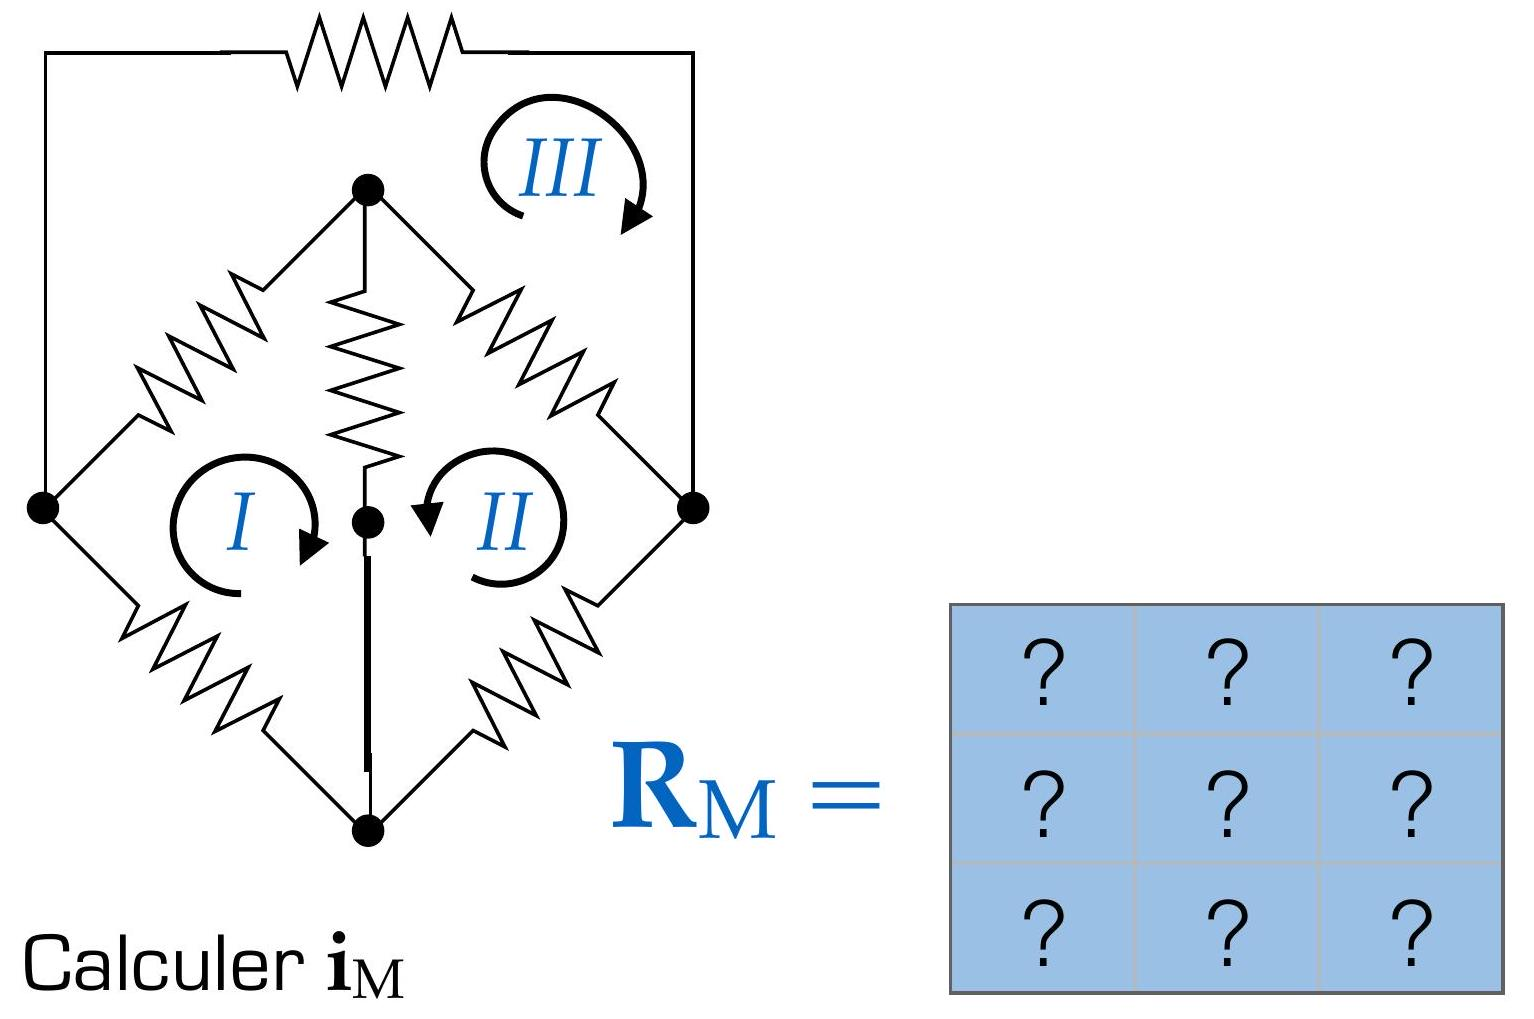
\includegraphics[max width=\textwidth, alt={}, center]{cbd435a9-cec2-4dd4-b13c-7b225dcc6548-12_1019_1534_343_1843}
\end{enumerate}

\begin{figure}[h]
\begin{center}
  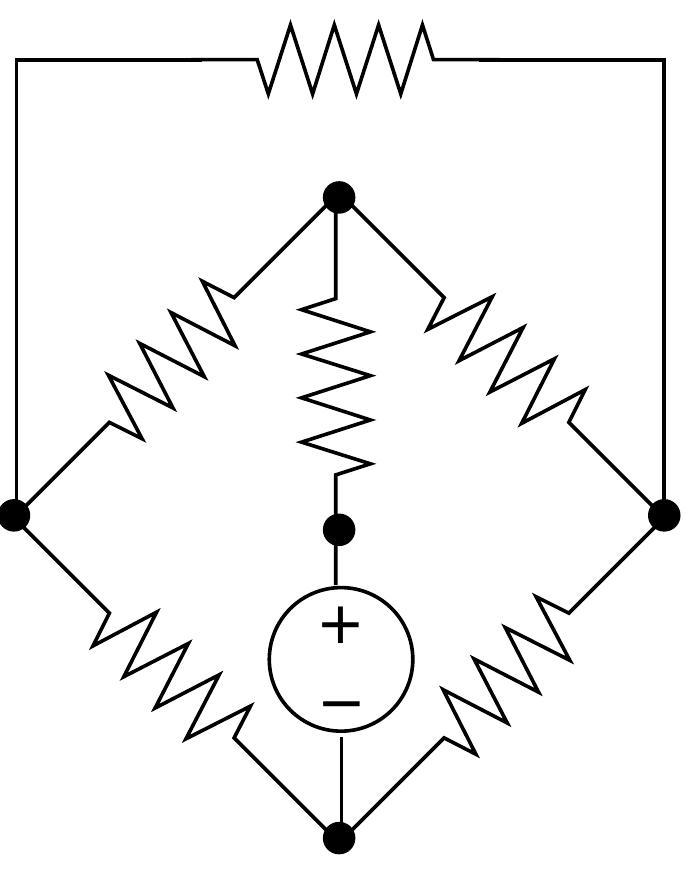
\includegraphics[alt={},max width=\textwidth]{cbd435a9-cec2-4dd4-b13c-7b225dcc6548-12_875_698_1384_1872}
\captionsetup{labelformat=empty}
\caption{$\dot{\mathbf{1}}_{\mathrm{M}}=\left(\dot{i}_{I}, \dot{i}_{I I}, \dot{i}_{I I I}\right)$}
\end{center}
\end{figure}

\section*{Conditions d'application}
\begin{itemize}
  \item Circuit linéaire
  \item Sources indépendantes de tension seulement
  \item Nous verrons plus tard comment gérer les sources indépendantes de courant et les source commandées de courant [CVT]
\end{itemize}

\section*{Dérivation de la méthode des mailles}
\begin{center}
\begin{tabular}{|l|l|l|}
\hline
[1] & $\mathbf{B u}_{\mathrm{B}}=\mathbf{v}_{\mathrm{s} \mathrm{M}}$ & SLK sur base de la matrice des mailles B \\
\hline
[ʔ] & $\mathbf{i}_{\mathrm{B}}=\mathbf{B}^{\mathrm{T}} \mathbf{i}_{\mathrm{M}}$ & Définition des courants de branches à partir des courants de maille et de B \\
\hline
[3] & $\mathbf{u}_{\mathrm{B}}=\mathbf{R}_{\mathrm{B}} \mathbf{i}_{\mathrm{B}}$ & Loi d'Ohm, via la matrice de résistances de branches \\
\hline
[4] & $\mathbf{B R}_{\mathbf{B}} \mathbf{i}_{\mathbf{B}}=\mathbf{v}_{\mathrm{SM}}$ & [1] dans [3] \\
\hline
[5] & $\mathbf{B R}_{\mathrm{B}} \mathbf{B}^{\mathrm{T}} \mathbf{i}_{\mathrm{M}}=\mathbf{v}_{\mathrm{s} \mathrm{M}}$ & [2] dans [4] \\
\hline
[6] & $\mathbf{B R}_{\mathrm{B}} \mathbf{B}^{\mathrm{T}}=\mathbf{R}_{\mathrm{M}}$ & Définition de la matrice de résistances de mailles \\
\hline
[7] & $\mathbf{R}_{\mathrm{M}} \mathbf{i}_{\mathrm{M}}=\mathbf{v}_{\mathrm{SM}}$ & [5] dans [6]: Résultat final \\
\hline
\end{tabular}
\end{center}

\section*{1a. La matrice des mailles B}
Formulation duale à celle de la matrice d'incidence.\\
Repose sur l'utilisation :

\begin{itemize}
  \item de la SLK écrite pour $b-(n-1)$ mailles fondamentales
  \item de la matrice des mailles fondamentales du graphe du circuit qui caractérise les relations mailles-branches du circuit
\end{itemize}

\section*{A. Seconde loi de Kirchhoff}
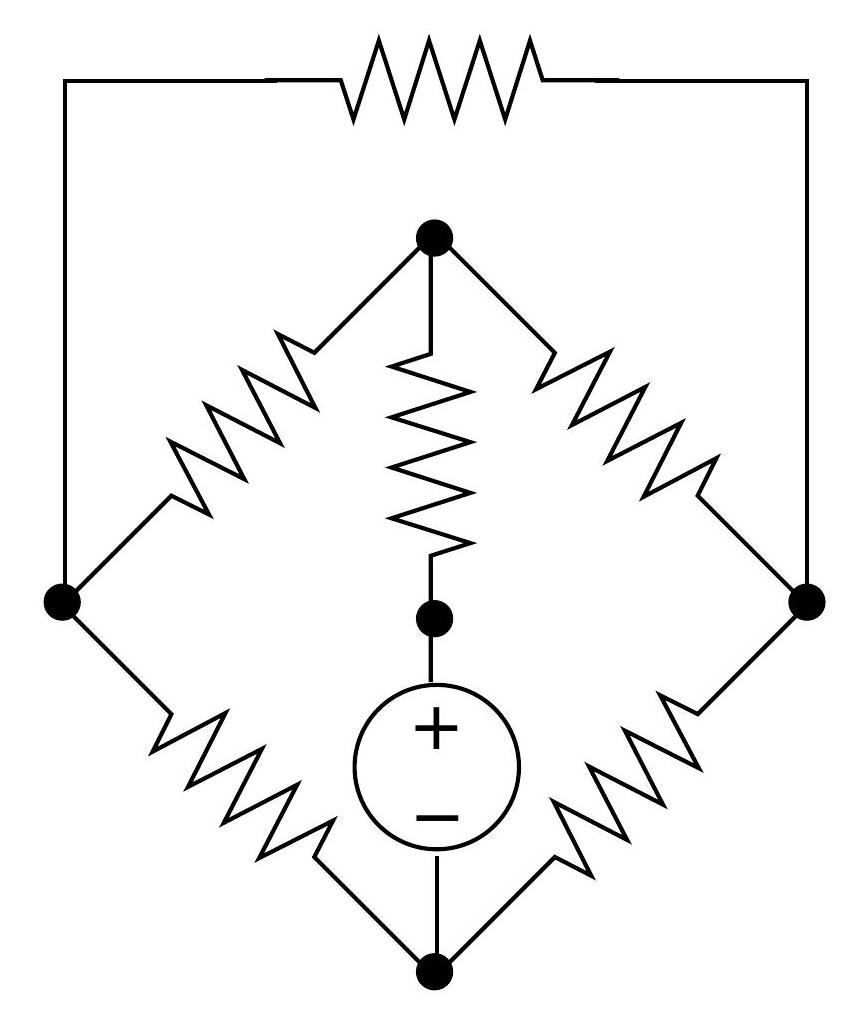
\includegraphics[max width=\textwidth, alt={}, center]{cbd435a9-cec2-4dd4-b13c-7b225dcc6548-16_1028_866_420_362}\\
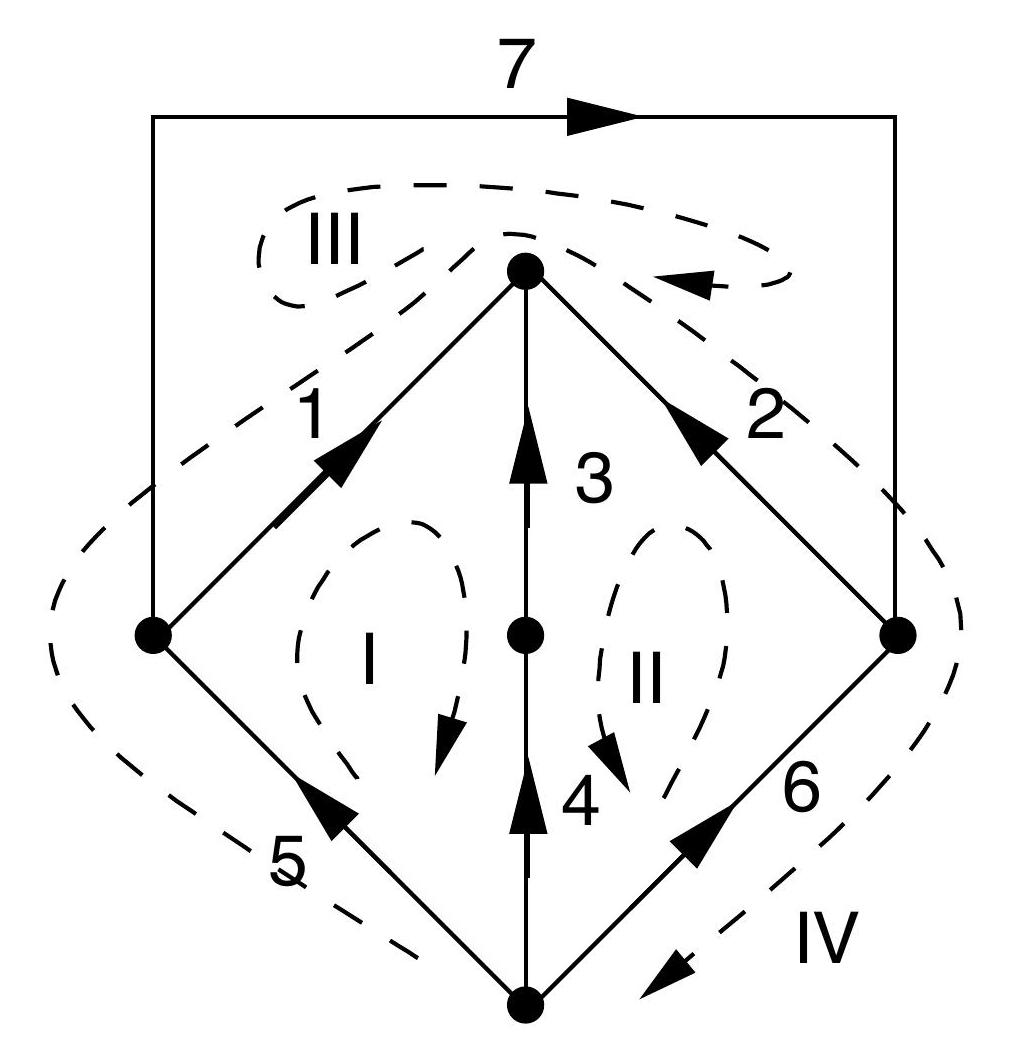
\includegraphics[max width=\textwidth, alt={}, center]{cbd435a9-cec2-4dd4-b13c-7b225dcc6548-16_1062_1013_405_1805}

\begin{center}
\begin{tabular}{|l|l|l|l|l|l|l|l|l|l|l|l|l|l|l|l|l|l|}
\hline
I &  &  &  & \multicolumn{2}{|c|}{} & $+$ &  & + & 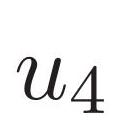
\includegraphics[max width=\textwidth, alt={}]{cbd435a9-cec2-4dd4-b13c-7b225dcc6548-16_134_123_1533_1627}
 &  &  & \multicolumn{2}{|c|}{} &  & $=$ &  & (1) \\
\hline
$\_\_\_\_$ &  & \multicolumn{2}{|c|}{} & $\_\_\_\_$ &  & $+$ &  & $+$ & $u_{4}$ &  &  & - & $u_{6}$ &  & \multicolumn{2}{|c|}{$=0$} & (2) \\
\hline
III & 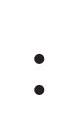
\includegraphics[max width=\textwidth, alt={}]{cbd435a9-cec2-4dd4-b13c-7b225dcc6548-16_117_68_1793_305}
 &  & $u_{1}$ & - & $u_{2}$ &  &  &  &  & \multicolumn{4}{|c|}{} & — \( u_{7} \) &  & $=0$ & (3) \\
\hline

\includegraphics[max width=\textwidth, alt={}]{cbd435a9-cec2-4dd4-b13c-7b225dcc6548-16_98_147_1945_105}
 &  &  &  &  & $u_{2}$ &  &  &  &  & - & $u_{5}$ & + & $u_{6}$ &  & $=$ & 0 & (4) \\
\hline
\end{tabular}
\end{center}

$$
-\mathbf{B}_{a} \mathbf{u}_{B}=\mathbf{0} \quad \text { ou } \quad \mathbf{B}_{a} \mathbf{u}_{B}=\mathbf{0}
$$

$\mathbf{B}_{a}$ : matrice des mailles du graphe orienté : matrice d'ordre $m \times b$\\
$m$ est le nombre total de mailles du circuit\\
En général, pas d'expression analytique simple en fonction de $n$ et $b$\\
$b_{i j}=+1 \quad$ si la branche $j$ appartient à la maille $i$ et est orientée dans le même sens\\
$b_{i j}=-1 \quad$ si la branche $j$ appartient à la maille $i$ et est orientée en sens inverse\\
$b_{i j}=0 \quad$ si la branche $j$ n'appartient pas à la maille $i$\\
$m$ relations linéairement dépendantes : par exemple (1)-(2) = (4)

\section*{Matrice des mailles fondamentales B}
Si l'on choisit uniquement un ensemble de mailles fondamentales, on obtient $b-(n-1)$ relations indépendantes.\\
Soit B la matrice des mailles fondamentales :\\
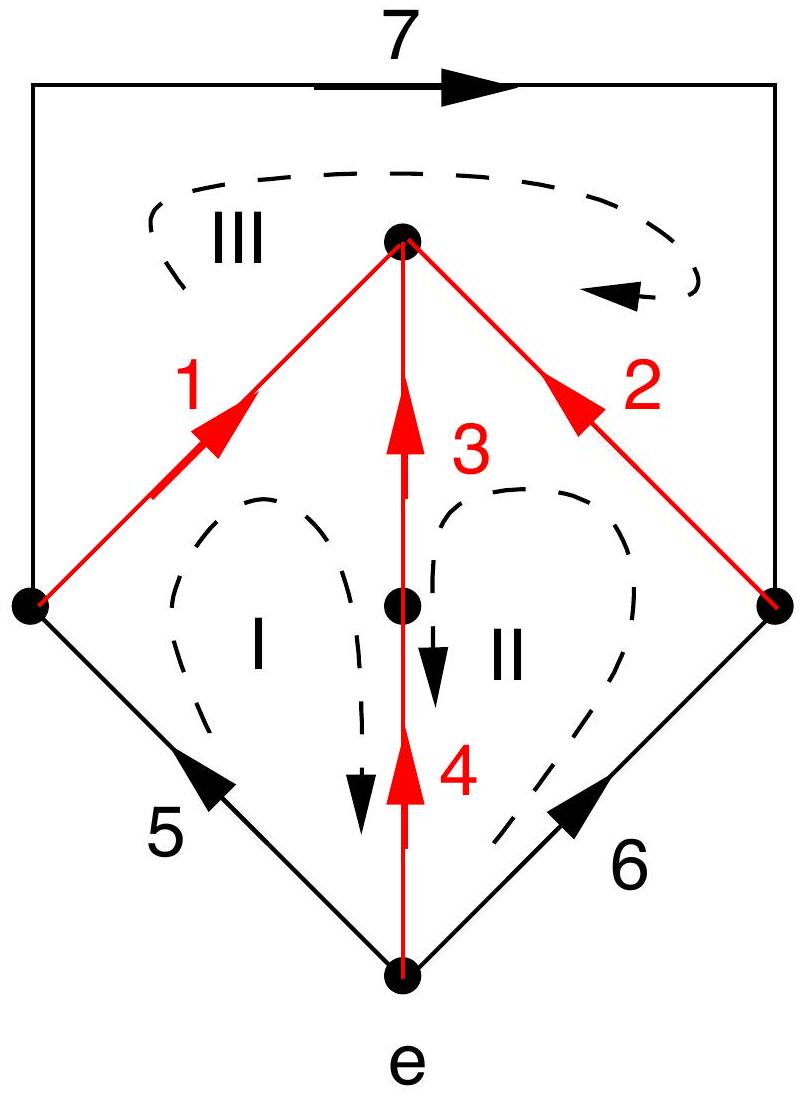
\includegraphics[max width=\textwidth, alt={}, center]{cbd435a9-cec2-4dd4-b13c-7b225dcc6548-18_1095_803_668_563}

$$
\mathbf{B}=\left[\begin{array}{rrrrrrr}
1 & 0 & -1 & -1 & 1 & 0 & 0 \\
0 & 1 & -1 & -1 & 0 & 1 & 0 \\
-1 & 1 & 0 & 0 & 0 & 0 & 1
\end{array}\right]
$$

SLK sous forme matricielle :\\
$\mathbf{B} \mathbf{u}_{B}=\mathbf{0}, b-(n-1)$ relations linéairement indépendantes

\section*{1b. Vecteur $\mathbf{v}_{s \mathrm{M}}$}
\begin{center}
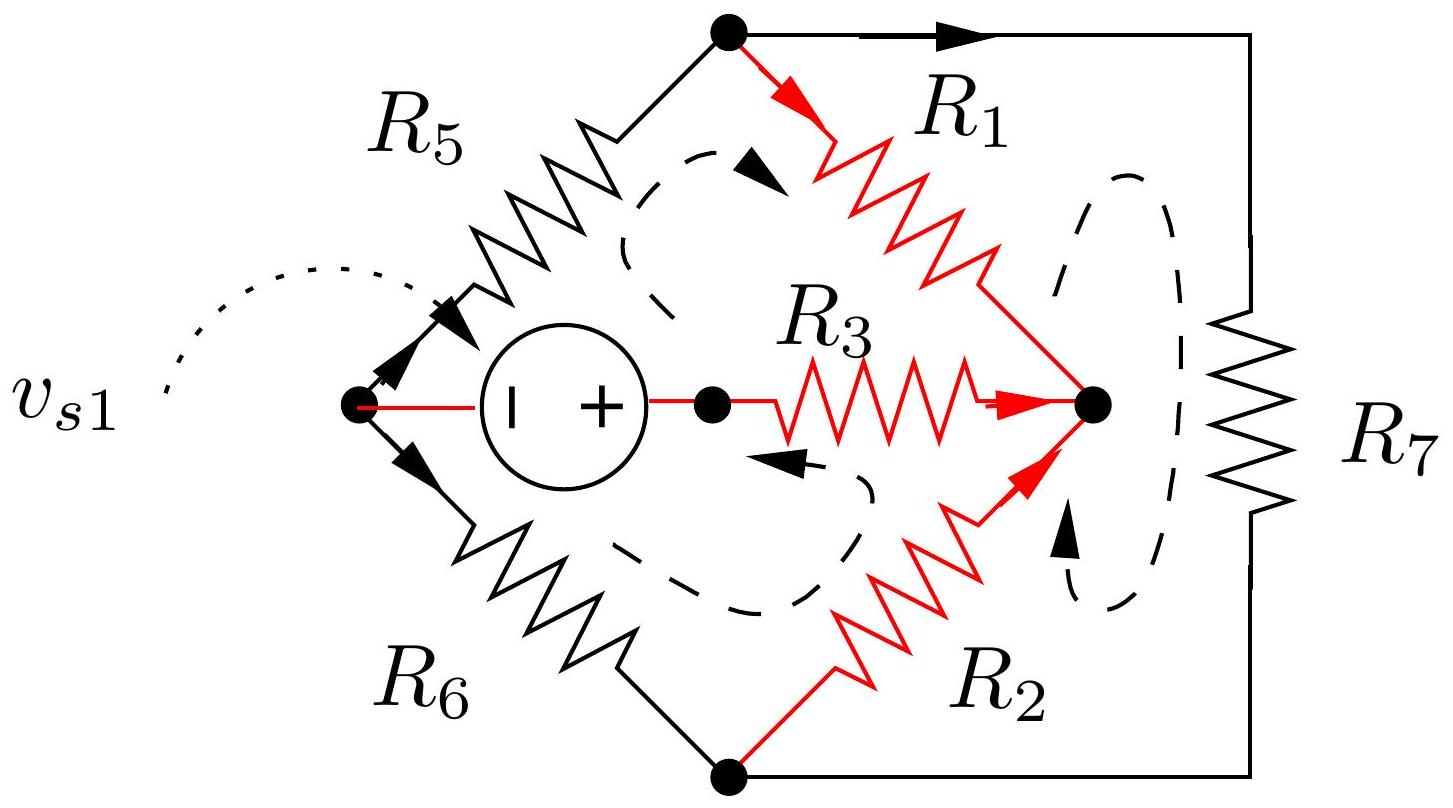
\includegraphics[max width=\textwidth, alt={}]{cbd435a9-cec2-4dd4-b13c-7b225dcc6548-19_808_1453_563_1155}
\end{center}

\begin{enumerate}
  \item SLK dans les $b-(n-1)$ mailles fondamentales
\end{enumerate}

$$
\begin{array}{lrl}
I: & u_{1}-u_{3}+u_{5} & =-v_{s 1} \\
I I: & u_{2}-u_{3}+u_{6} & =-v_{s 1} \\
I I I: & -u_{1}+u_{2}+u_{7} & =0
\end{array} \quad \Longleftrightarrow \mathbf{B} \mathbf{~ u}_{B}=\mathbf{v}_{s M}
$$

B : matrice des mailles fondamentales du circuit passifié = circuit où l'on a rendues inactives toutes les sources indépendantes d'énergie.\\
Sources indépendantes de tension, $v=0$ : remplacer par un court-circuit\\
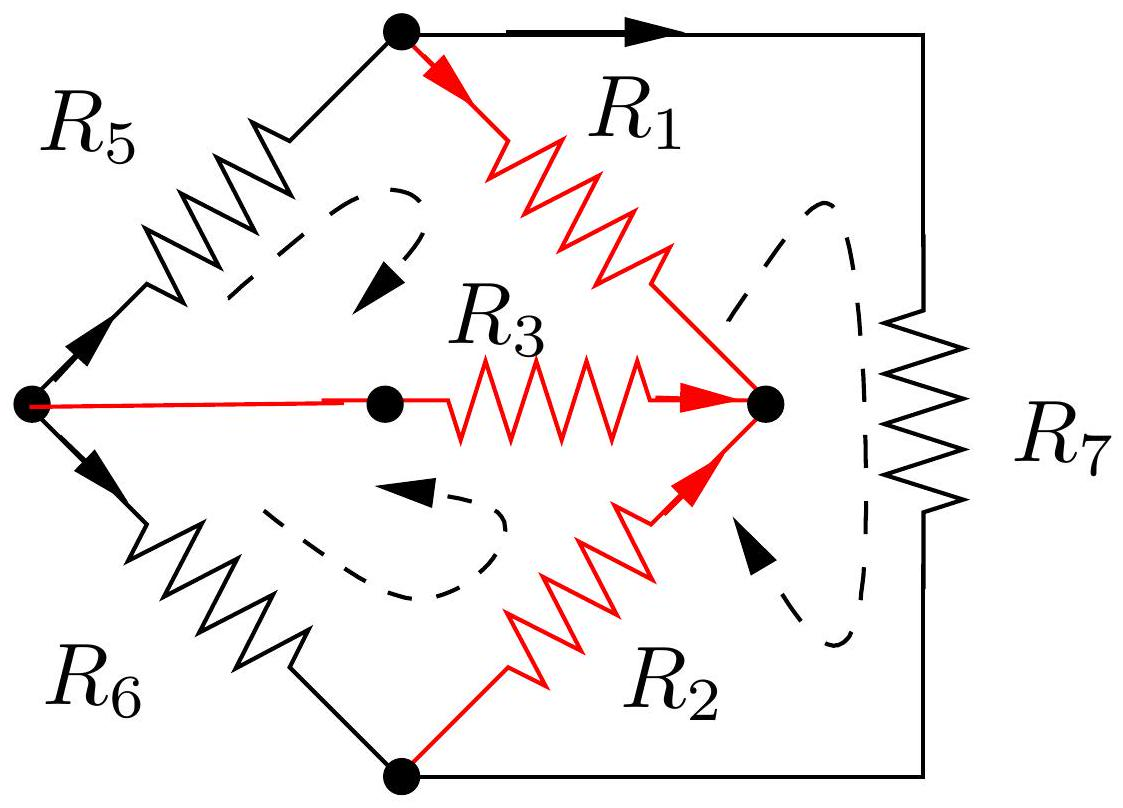
\includegraphics[max width=\textwidth, alt={}, center]{cbd435a9-cec2-4dd4-b13c-7b225dcc6548-20_808_1123_926_210}

$$
\mathbf{B}=\left[\begin{array}{rrrrrr}
1 & 0 & -1 & 1 & 0 & 0 \\
0 & 1 & -1 & 0 & 1 & 0 \\
-1 & 1 & 0 & 0 & 0 & 1
\end{array}\right]
$$

Vecteur $\mathbf{i}_{M}$ des courants dans les maillons : $\mathbf{i}_{M}=\left[i_{5}, i_{6}, i_{7}\right]^{T}$\\
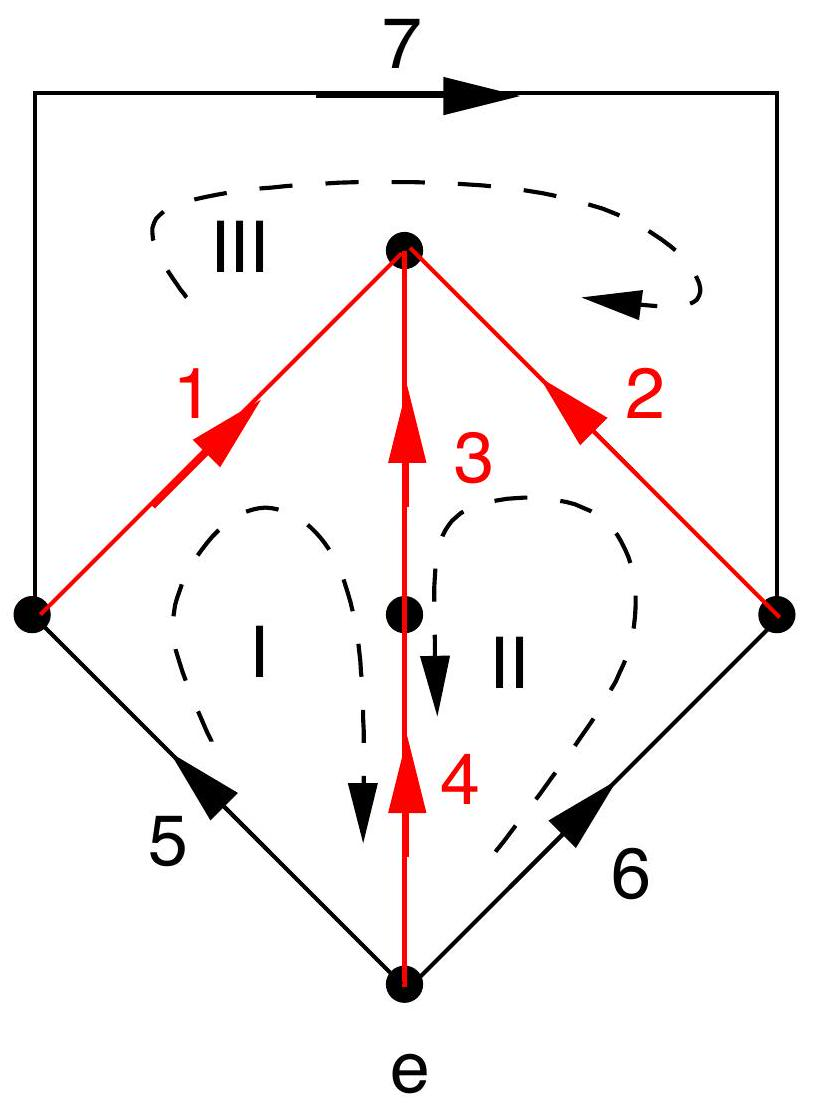
\includegraphics[max width=\textwidth, alt={}, center]{cbd435a9-cec2-4dd4-b13c-7b225dcc6548-21_1109_813_702_210}

$$
\left[\begin{array}{l}
i_{1} \\
i_{2} \\
i_{3} \\
i_{4} \\
i_{5} \\
i_{6} \\
i_{7}
\end{array}\right]=\left[\begin{array}{rrr}
1 & 0 & -1 \\
0 & 1 & 1 \\
-1 & -1 & 0 \\
-1 & -1 & 0 \\
1 & 0 & 0 \\
0 & 1 & 0 \\
0 & 0 & 1
\end{array}\right]\left[\begin{array}{c}
i_{I} \\
i_{I I} \\
i_{I I I}
\end{array}\right]
$$

PLK sous forme matricielle :

$$
\mathbf{i}_{B}=\mathbf{B}^{T} \mathbf{i}_{M}
$$

\section*{Matrices de résistances de mailles $\mathbf{R}_{\mathrm{M}}$}
Appliquer la loi d'Ohm dans chaque branche (relation $u=f(i)$ ) : permet de remplacer $\mathbf{u}_{B} \operatorname{par} \mathbf{i}_{B}$

$$
\begin{aligned}
u_{1}=R_{1} i_{1}, \quad u_{2}=R_{2} i_{2}, & \ldots, \quad u_{7}=R_{7} i_{7} \\
R_{1} i_{1}-R_{3} i_{3}+R_{5} i_{5} & =-v_{s 1} \\
R_{2} i_{2}-R_{3} i_{3}+R_{6} i_{6} & =-v_{s 1} \quad \Longleftrightarrow \quad \mathbf{u}_{B}=\mathbf{R}_{B} \mathbf{i}_{B} \\
-R_{1} i_{1}+R_{2} i_{2}+R_{7} i_{7} & =0
\end{aligned}
$$

$\mathbf{R}_{B}$ : matrice de résistances de branches

$$
\mathbf{R}_{B}=\left[\begin{array}{cccc}
R_{1} & & & \\
& R_{2} & \mathbf{0} & \\
& \mathbf{0} & \ddots & \\
& & & R_{7}
\end{array}\right] \quad \begin{aligned}
& \text { matrice diagonale } \\
& \text { linéaires uniquement }
\end{aligned}
$$

si résistances\\
si 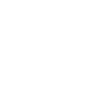
\includegraphics[max width=\textwidth, alt={}]{image-not-found}

\section*{C. PLK et courants de mailles}
On remplace les courants de branches $\mathbf{i}_{B}$ par les courants de mailles $\mathbf{i}_{M}$ via la PLK

$$
\begin{aligned}
i_{1}=i_{M 1}-i_{M 3} \quad i_{2}=i_{M 2}+i_{M 3} \quad \ldots \quad i_{7}=i_{M 3} & \Longleftrightarrow \mathbf{i}_{B}=\mathbf{B}^{T} \mathbf{i}_{M} \\
\left(R_{1}+R_{3}+R_{5}\right) i_{M 1}+R_{3} i_{M 2}-R_{1} i_{M 3} & =-v_{s 1} \\
R_{3} i_{M 1}+\left(R_{2}+R_{3}+R_{6}\right) i_{M 2}+R_{2} i_{M 3} & =-v_{s 1} \\
-R_{1} i_{M 1}+R_{2} i_{M 2}+\left(R_{1}+R_{2}+R_{7}\right) i_{M 3} & =0 \\
\Longleftrightarrow &
\end{aligned}
$$

$$
\underbrace{\mathbf{B R}_{B} \mathbf{B}^{T}}_{\mathbf{R}_{M}} \mathbf{i}_{M}=\mathbf{v}_{s M}
$$

\section*{3. Matrice de résistances de mailles}
$$
\mathbf{R}_{M}=\mathbf{B} \mathbf{R}_{B} \mathbf{B}^{T}=\left[\begin{array}{ccc}
R_{1}+R_{3}+R_{5} & R_{3} & -R_{1} \\
R_{3} & R_{2}+R_{3}+R_{6} & R_{2} \\
-R_{1} & R_{2} & R_{1}+R_{2}+R_{7}
\end{array}\right]
$$

\begin{center}
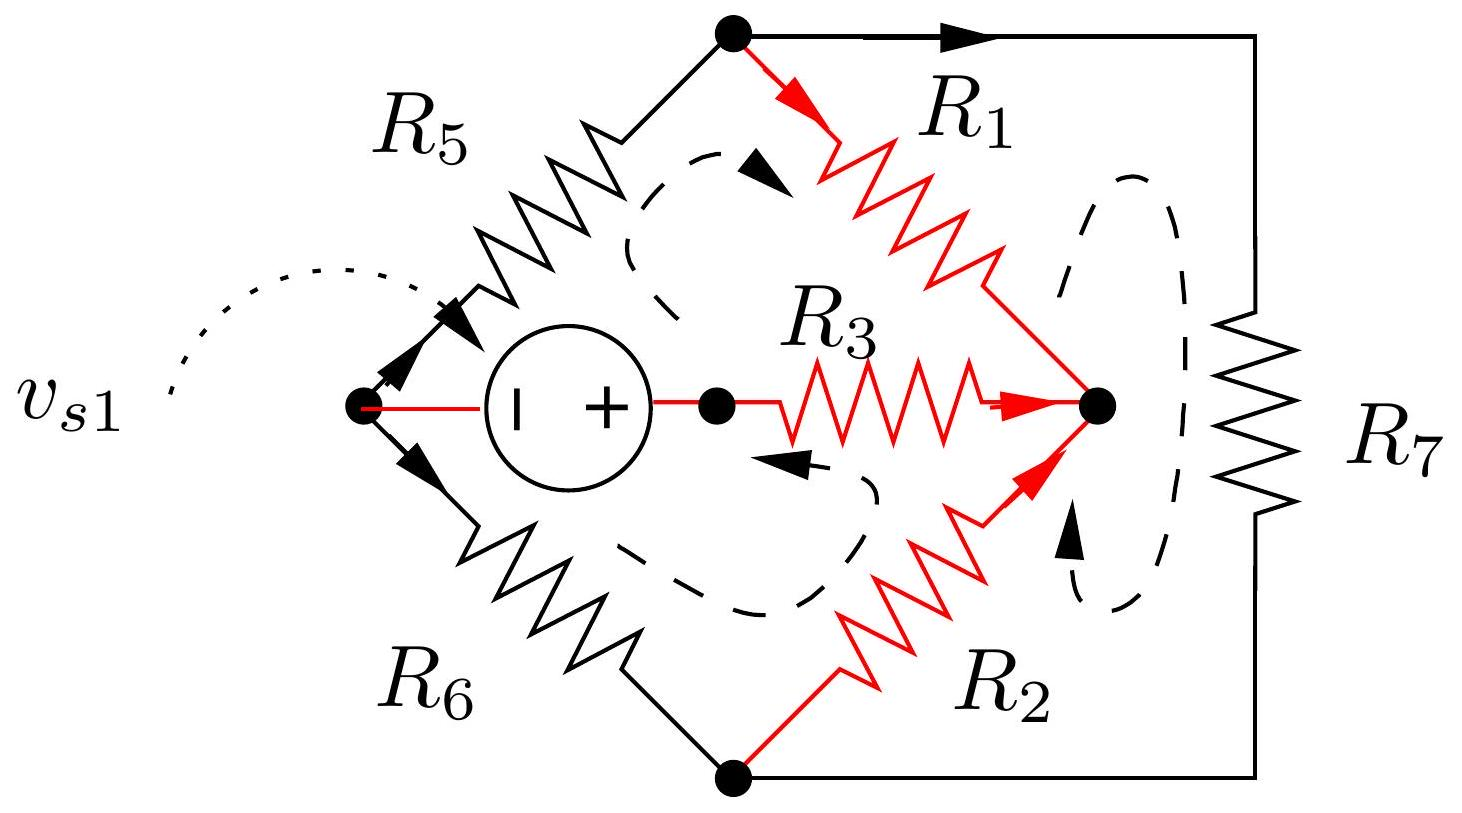
\includegraphics[max width=\textwidth, alt={}]{cbd435a9-cec2-4dd4-b13c-7b225dcc6548-24_813_1462_649_1041}
\end{center}

\section*{Détermination de $\mathbf{R}_{M}$ par inspection :}
\begin{itemize}
  \item $R_{i i}=$ somme des résistances des branches de la maille $i$
  \item $R_{i k}=$ somme des résistances des branches communes aux mailles $i$ et $k$, prises avec le signe + si les sens de parcours des deux mailles coïncident, avec le signe dans le cas contraire
\end{itemize}

\section*{Réseau équivalent}
Le circuit peut être remplacé par un circuit équivalent constitué du circuit passifié vu de $M=b-(n-1)$ accès auquels agissent des sources indépendantes de tension équivalentes regroupant les sources indépendantes du circuit original.\\
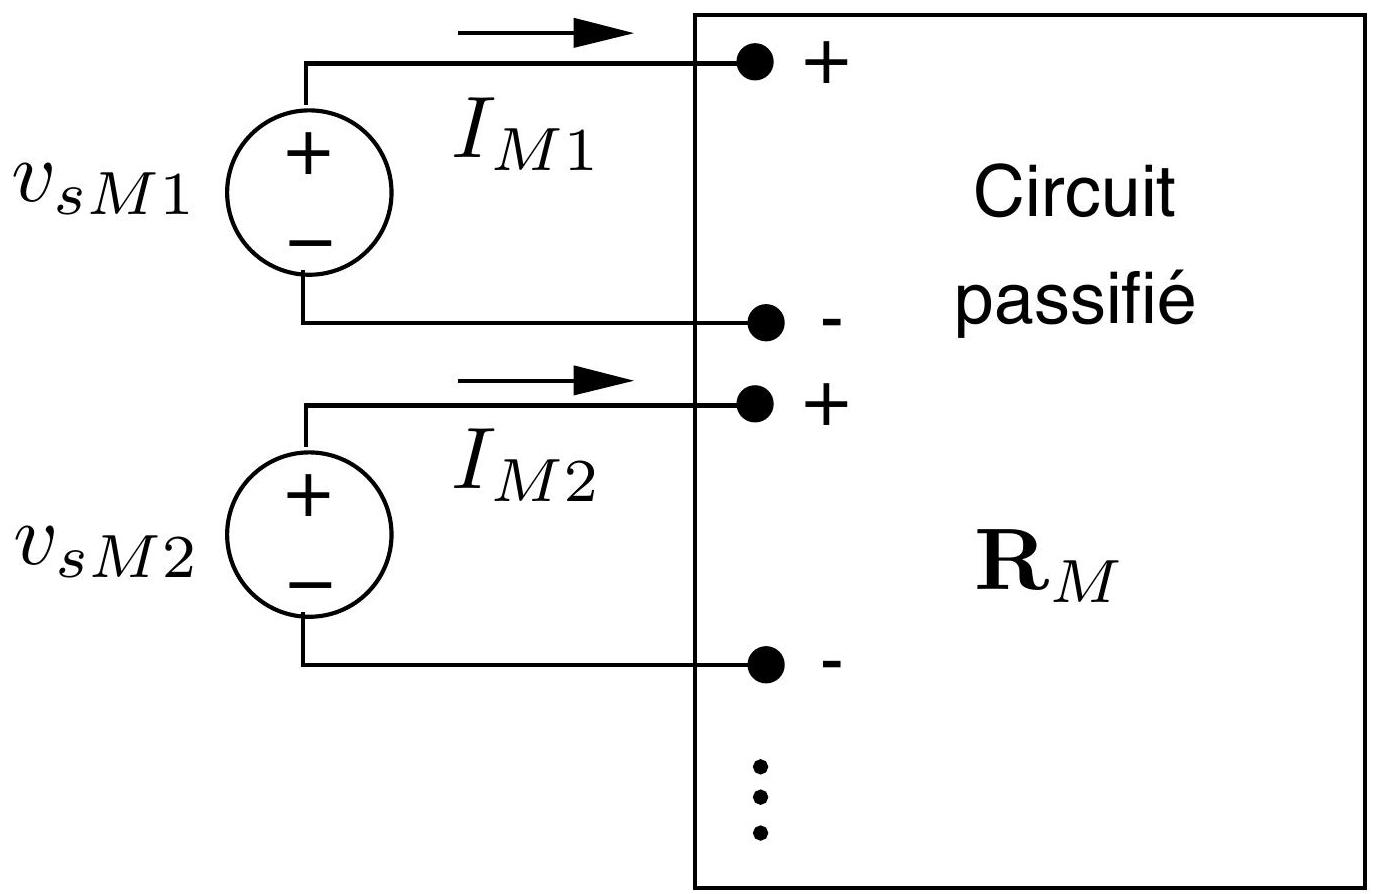
\includegraphics[max width=\textwidth, alt={}, center]{cbd435a9-cec2-4dd4-b13c-7b225dcc6548-25_894_1376_955_181}

Réseau passifié avec

\begin{itemize}
  \item un accès dans chaque maillon (on "ouvre" le maillon)
  \item une source indépendante de tension agissant à chaque accès qui "ferme" le maillon
\end{itemize}

\section*{Exemple}
\begin{center}
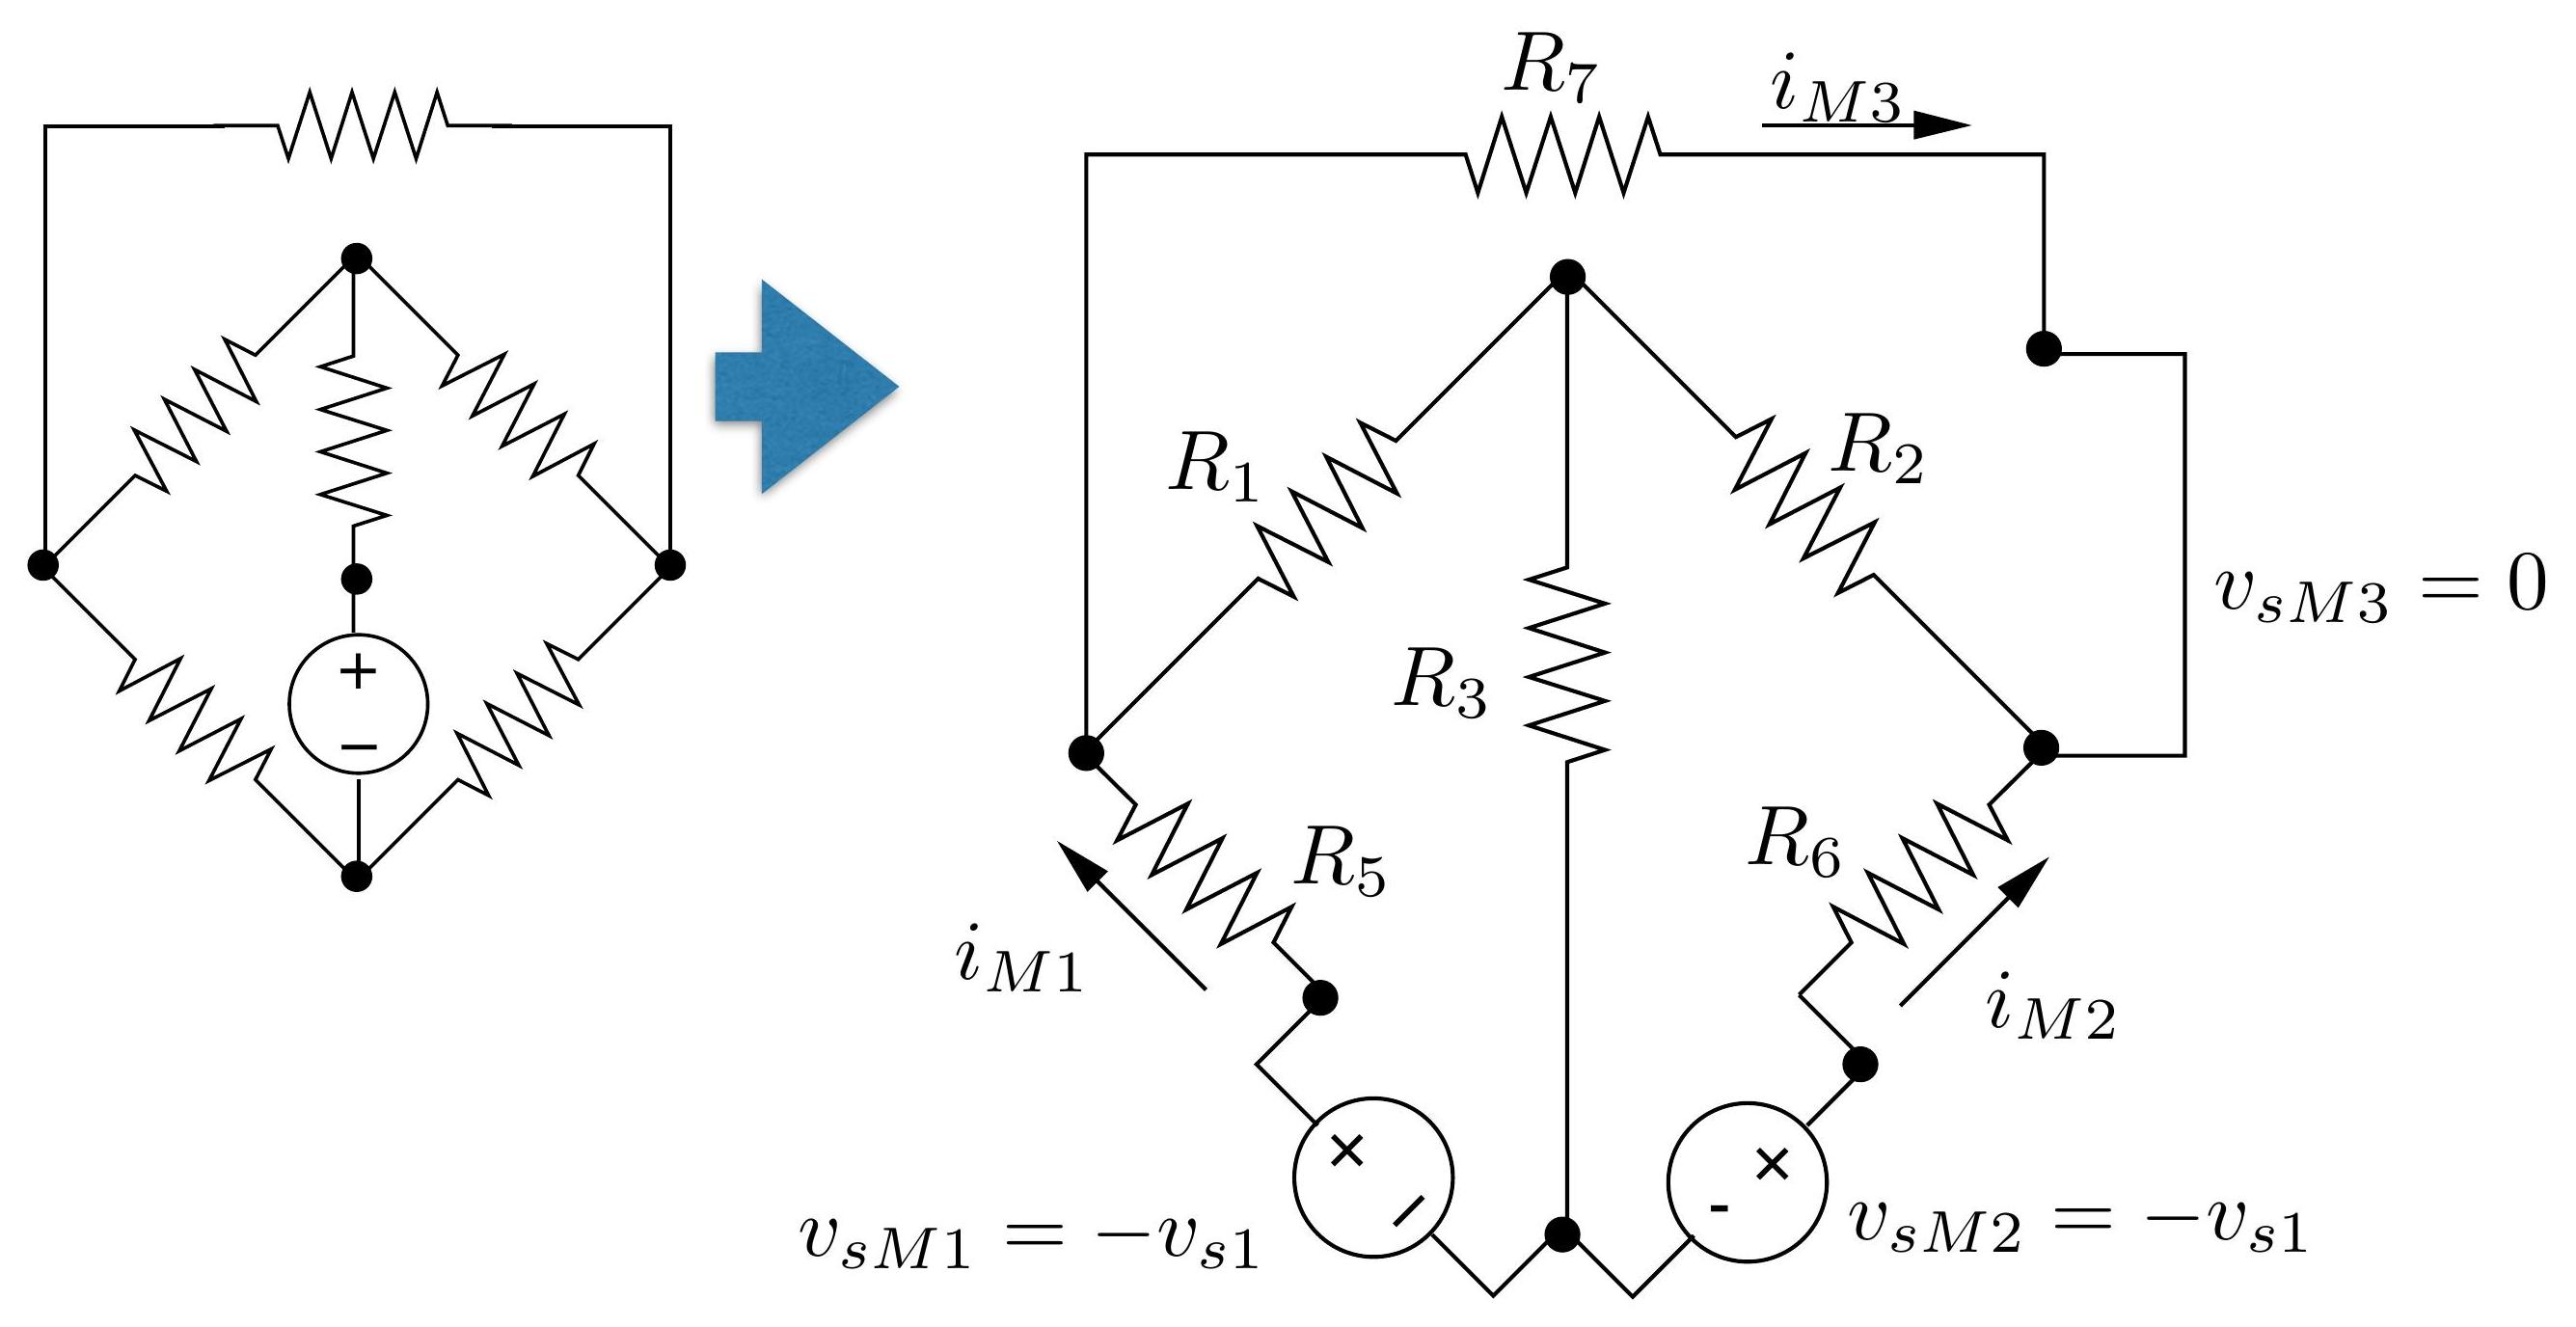
\includegraphics[max width=\textwidth, alt={}]{cbd435a9-cec2-4dd4-b13c-7b225dcc6548-26_1376_2671_525_85}
\end{center}

\section*{Et si le circuit comporte des sources commandées ?}
Source de type CVT uniquement, introduit une relation de branche du type $u=f(i)$ qui peut être facilement intégrée à l'étape B. (cfr. Dérivation) Autres types de sources commandées : pas toujours possible\\
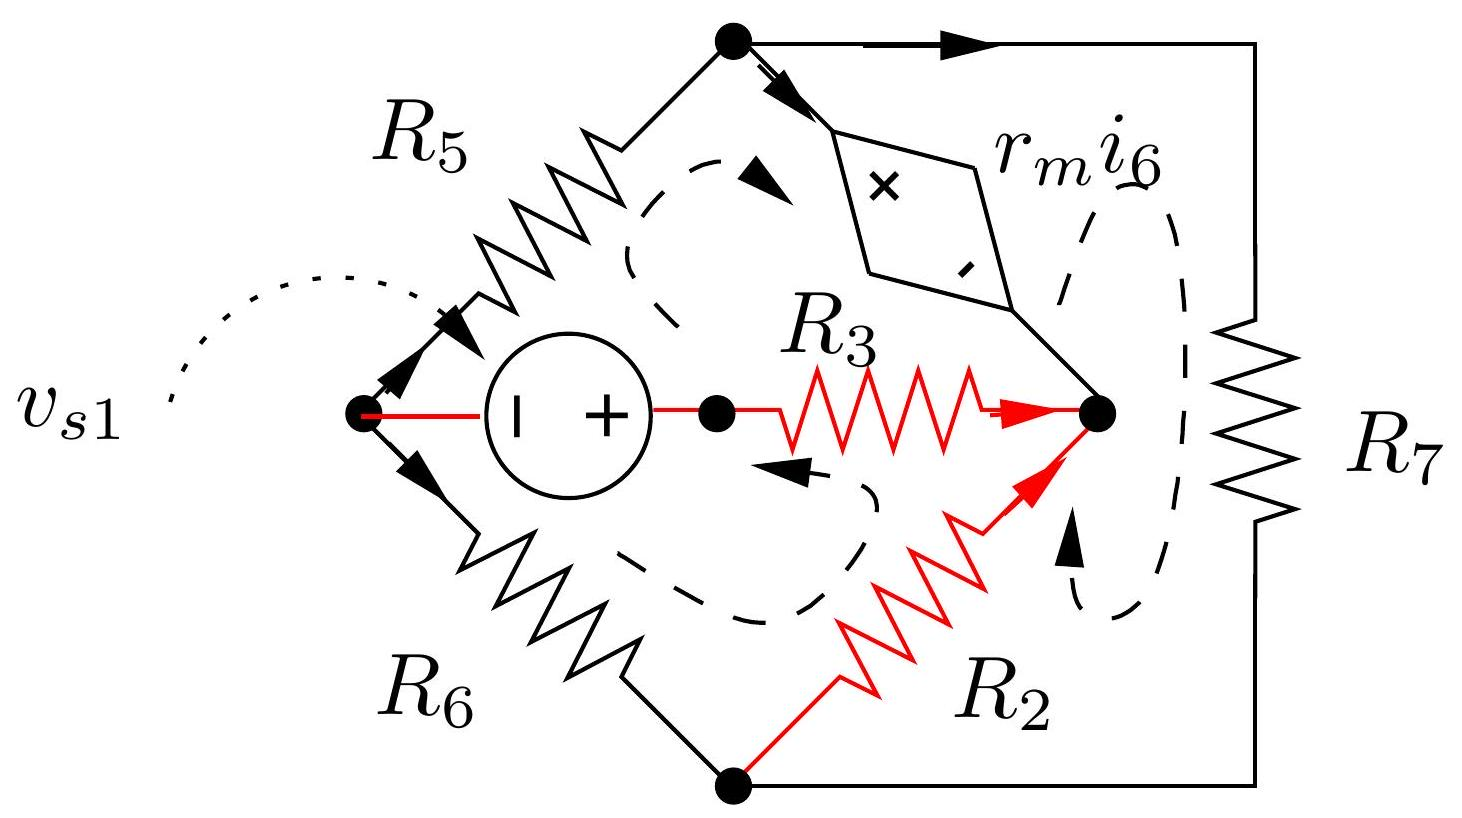
\includegraphics[max width=\textwidth, alt={}, center]{cbd435a9-cec2-4dd4-b13c-7b225dcc6548-27_818_1462_907_1041}

$$
\text { relation } u=f(i): \quad u_{1}=r_{m} i_{6}=r_{m} i_{M 2}
$$

SLK dans la maille $\mathrm{I}: R_{3}\left(i_{M 1}+i_{M 2}\right)+R_{5} i_{M 1}+r_{m} i_{M 2}=-v_{s 1}$\\
SLK dans la maille III : $R_{2}\left(i_{M 2}+i_{M 3}\right)+R_{7} i_{M 3}-r_{m} i_{M 2}=0$

Matrice de résistances de branches :

$$
\mathbf{R}_{B}=\left[\begin{array}{cccccc}
0 & 0 & 0 & 0 & r_{m} & 0 \\
0 & R_{2} & 0 & 0 & 0 & 0 \\
0 & 0 & R_{3} & 0 & 0 & 0 \\
0 & 0 & 0 & R_{5} & 0 & 0 \\
0 & 0 & 0 & 0 & R_{6} & 0 \\
0 & 0 & 0 & 0 & 0 & R_{7}
\end{array}\right]
$$

Matrice de résistances de mailles :

$$
\mathbf{R}_{M}=\mathbf{B} \mathbf{R}_{B} \mathbf{B}^{T}=\left[\begin{array}{ccc}
R_{3}+R_{5} & R_{3}+r_{m} & 0 \\
R_{3} & R_{2}+R_{3}+R_{6} & R_{2} \\
0 & R_{2}-r_{m} & R_{2}+R_{7}
\end{array}\right]
$$

Même matrice B que précédemment.\\
$\mathbf{R}_{B}$ et $\mathbf{R}_{M}$ ne sont plus des matrices symétriques. $\mathbf{R}_{M}$ ne peut plus être déterminée par inspection !!

\section*{Détermination de la matrice de résistance de mailles par expérimentation}
Utiliser le réseau équivalent; $\mathbf{R}_{M}$ caractérise le circuit passifié. Les relations $u-i$ aux $b-(n-1)$ accès s'écrivent :

$$
\begin{aligned}
& u_{1}=R_{11} i_{1}+R_{12} i_{2}+\ldots \\
& u_{2}=R_{21} i_{1}+R_{22} i_{2}+\ldots
\end{aligned}
$$

i est le vecteur des courants injectés aux accès, $\mathbf{v}$ est le vecteur des tensions aux accès.

Les éléments de $\mathbf{R}_{M}$ sont déterminés par des essais successifs :

$$
R_{i j}=\left.u_{i}\right|_{i_{j}=1, i_{k}=0, k \neq j}
$$

\begin{itemize}
  \item Imposer un courant de 1 A à l'accès $j$
  \item Laisser les autres accès ouverts ( $i=0$ )
  \item Déterminer dans ces conditions la tension à l'accès $i$
\end{itemize}

Elément diagonal :\\
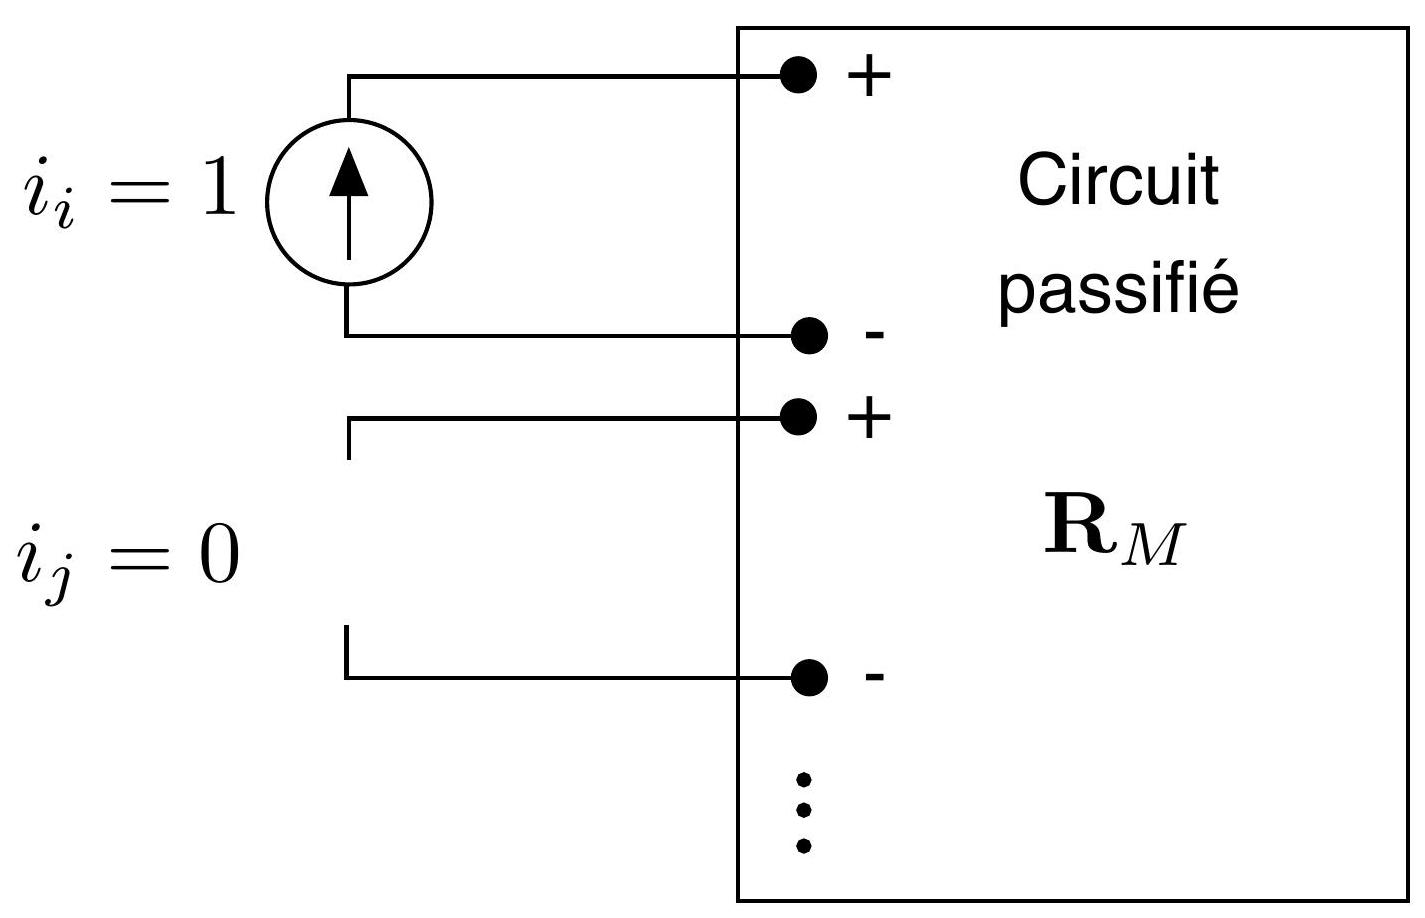
\includegraphics[max width=\textwidth, alt={}, center]{cbd435a9-cec2-4dd4-b13c-7b225dcc6548-30_918_1425_678_386}

$$
R_{i i}=\left.v_{i}\right|_{i_{i}=1, i_{k}=0, k \neq i}
$$

Tension à l'accès $i$ lorsque tous les accès sauf l'accès $i$ sont laissés ouverts.

Elément non-diagonal :\\
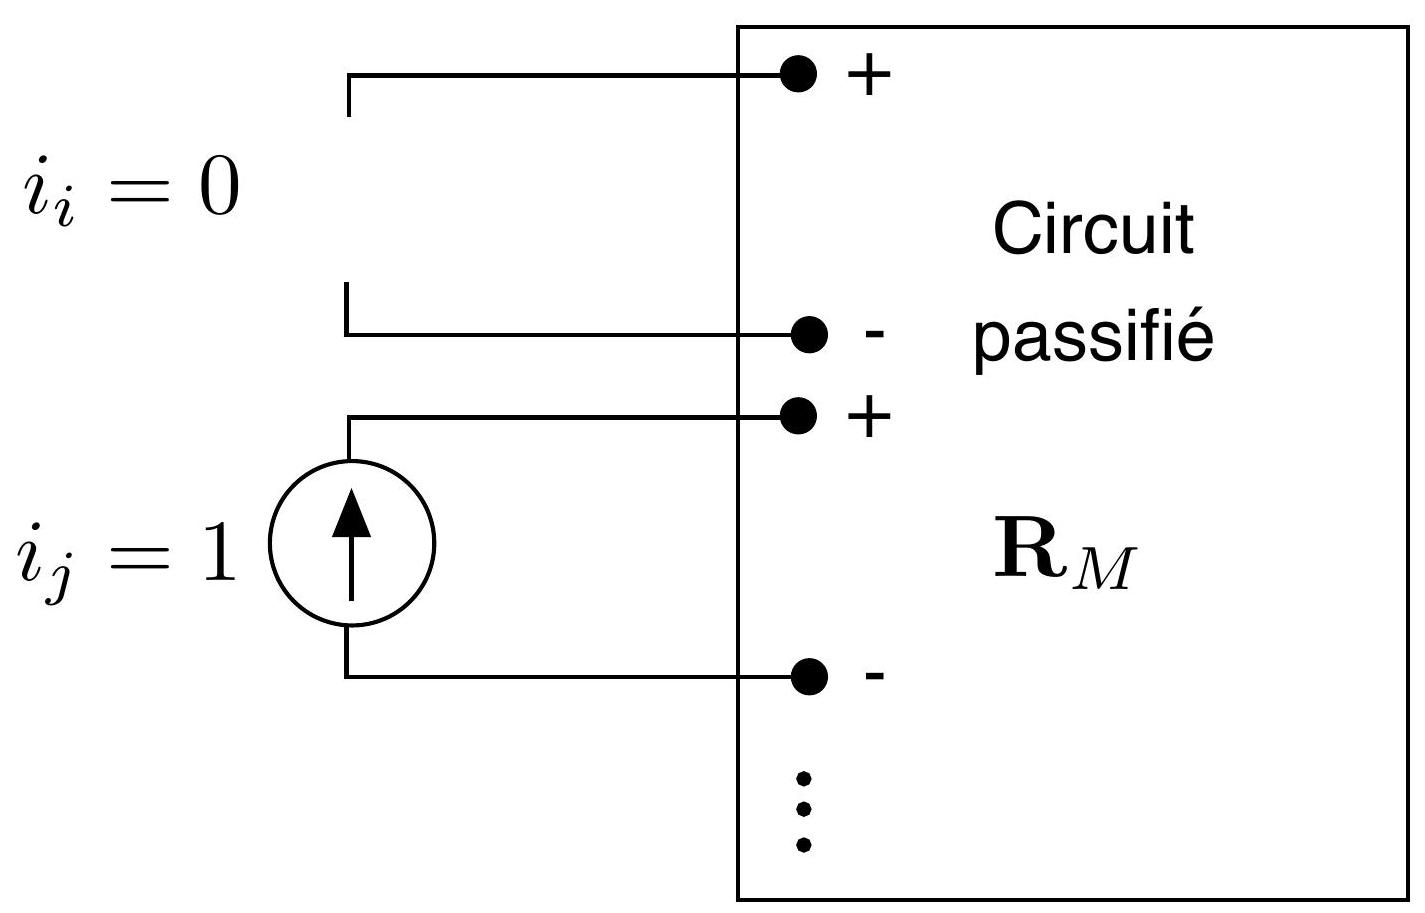
\includegraphics[max width=\textwidth, alt={}, center]{cbd435a9-cec2-4dd4-b13c-7b225dcc6548-31_913_1425_678_386}

$$
R_{i j}=\left.v_{i}\right|_{i_{j}=1, i_{k}=0, k \neq j}
$$

Tension à l'accès $i$ lorsque tous les accès sauf l'accès $j$ sont laissés ouverts.

$$
R_{11}=\left.v_{I}\right|_{i_{I}=1, i_{I I}=i_{I I I}=0}
$$

\begin{center}
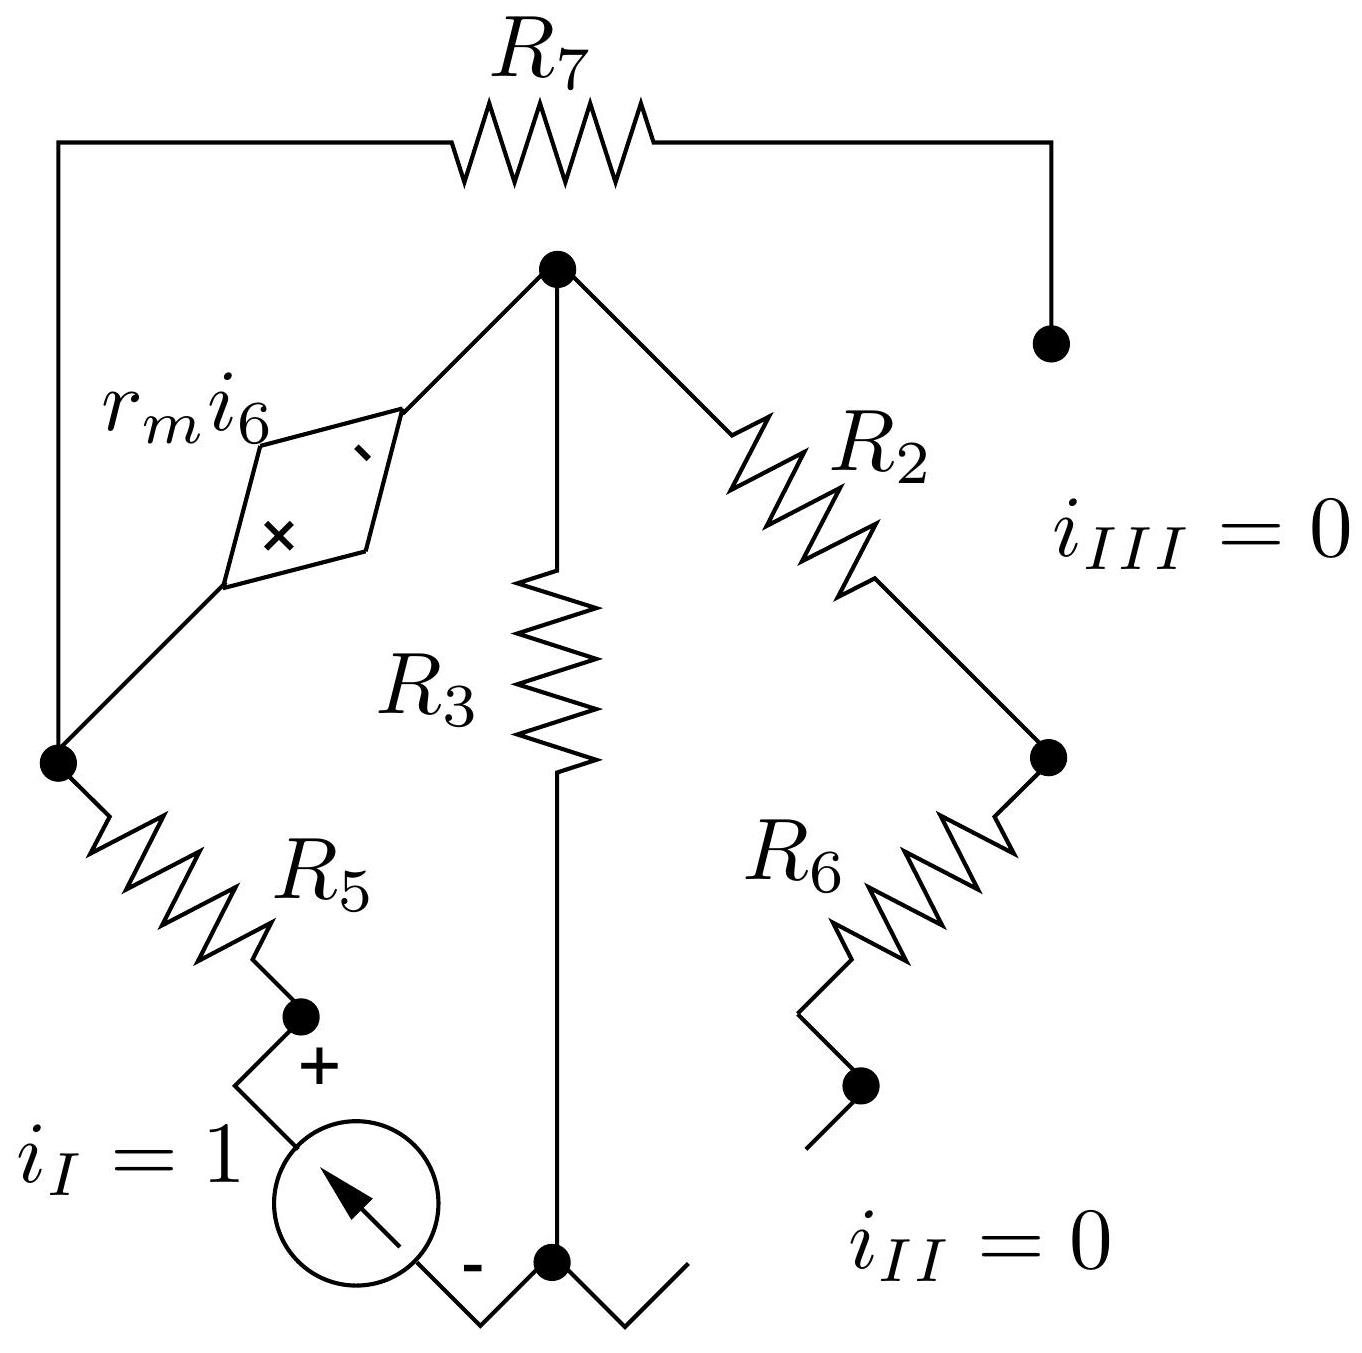
\includegraphics[max width=\textwidth, alt={}]{cbd435a9-cec2-4dd4-b13c-7b225dcc6548-32_1353_1362_601_659}
\end{center}

$$
\begin{aligned}
i_{6} & =0 \\
R_{11}=v_{I} & =R_{5}+R_{3}
\end{aligned}
$$

$$
R_{12}=\left.v_{I}\right|_{i_{I I}=1, i_{I}=i_{I I I}=0}
$$

\begin{center}
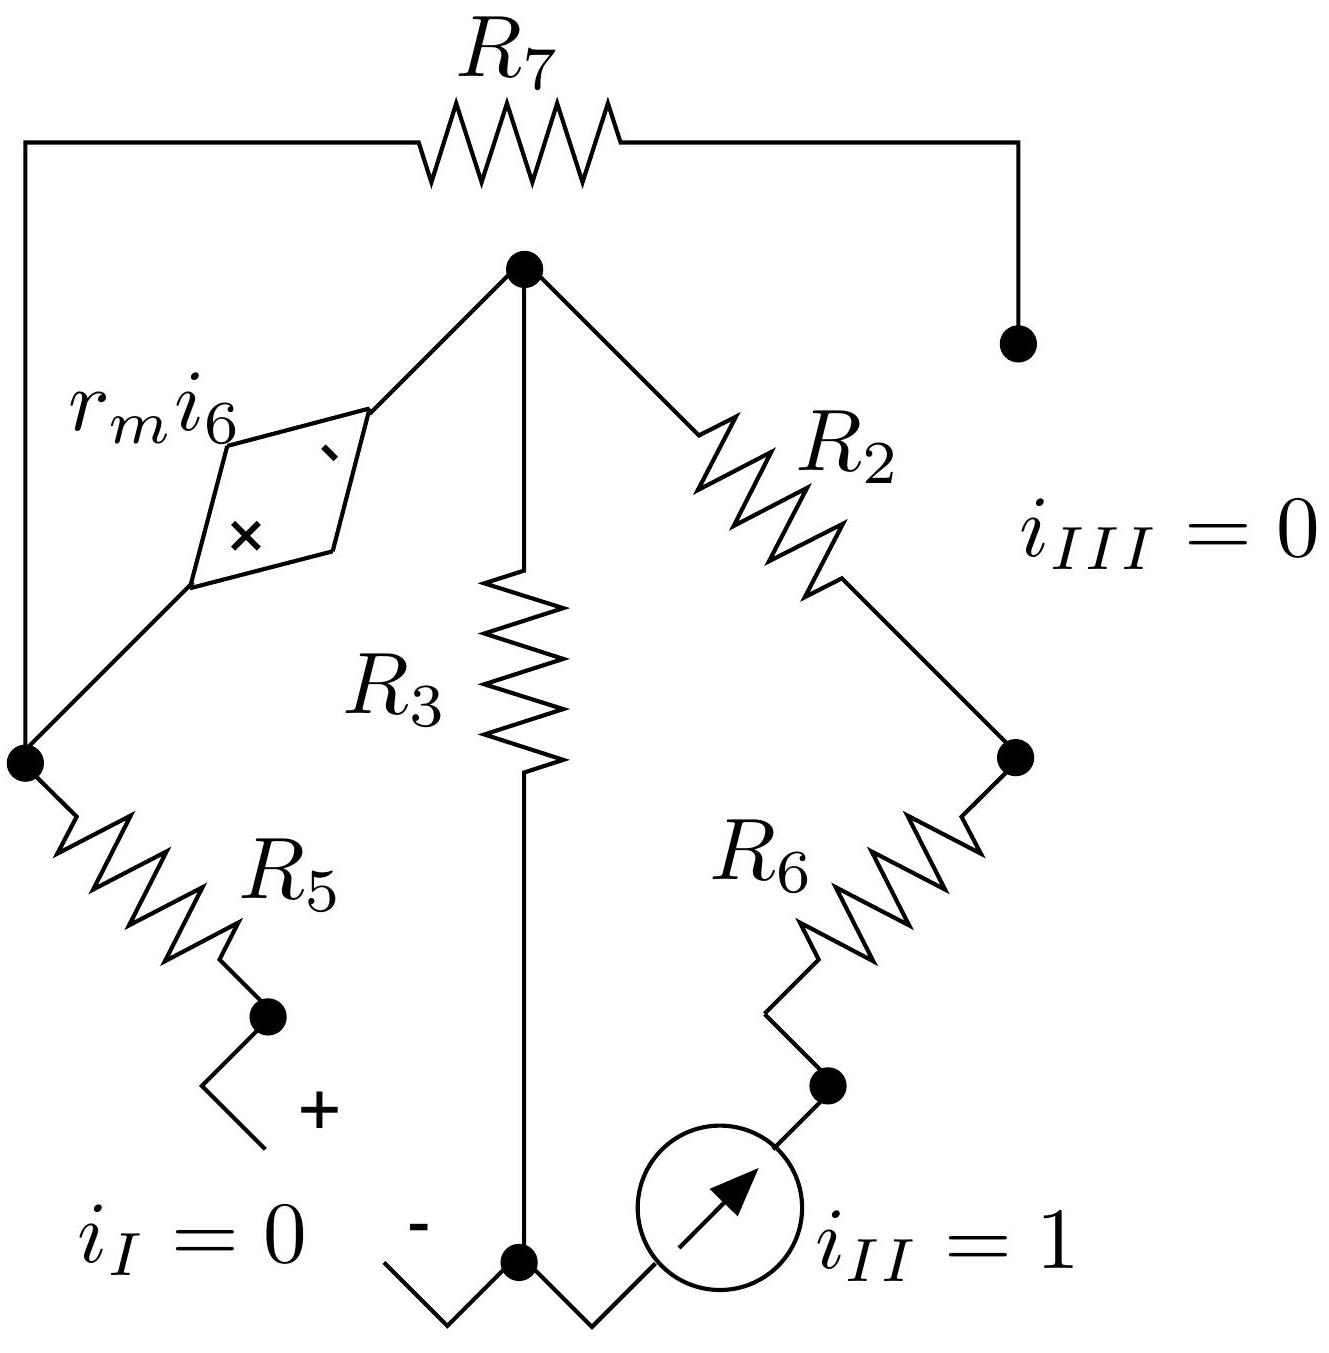
\includegraphics[max width=\textwidth, alt={}]{cbd435a9-cec2-4dd4-b13c-7b225dcc6548-33_1353_1329_601_692}
\end{center}

$$
\begin{aligned}
i_{5} & =0 \\
i_{6} & =1 \\
R_{12}=v_{I} & =R_{3}+r_{m}
\end{aligned}
$$

$$
R_{13}=\left.v_{I}\right|_{i_{I I I}=1, i_{I}=i_{I I}=0}
$$

\begin{center}
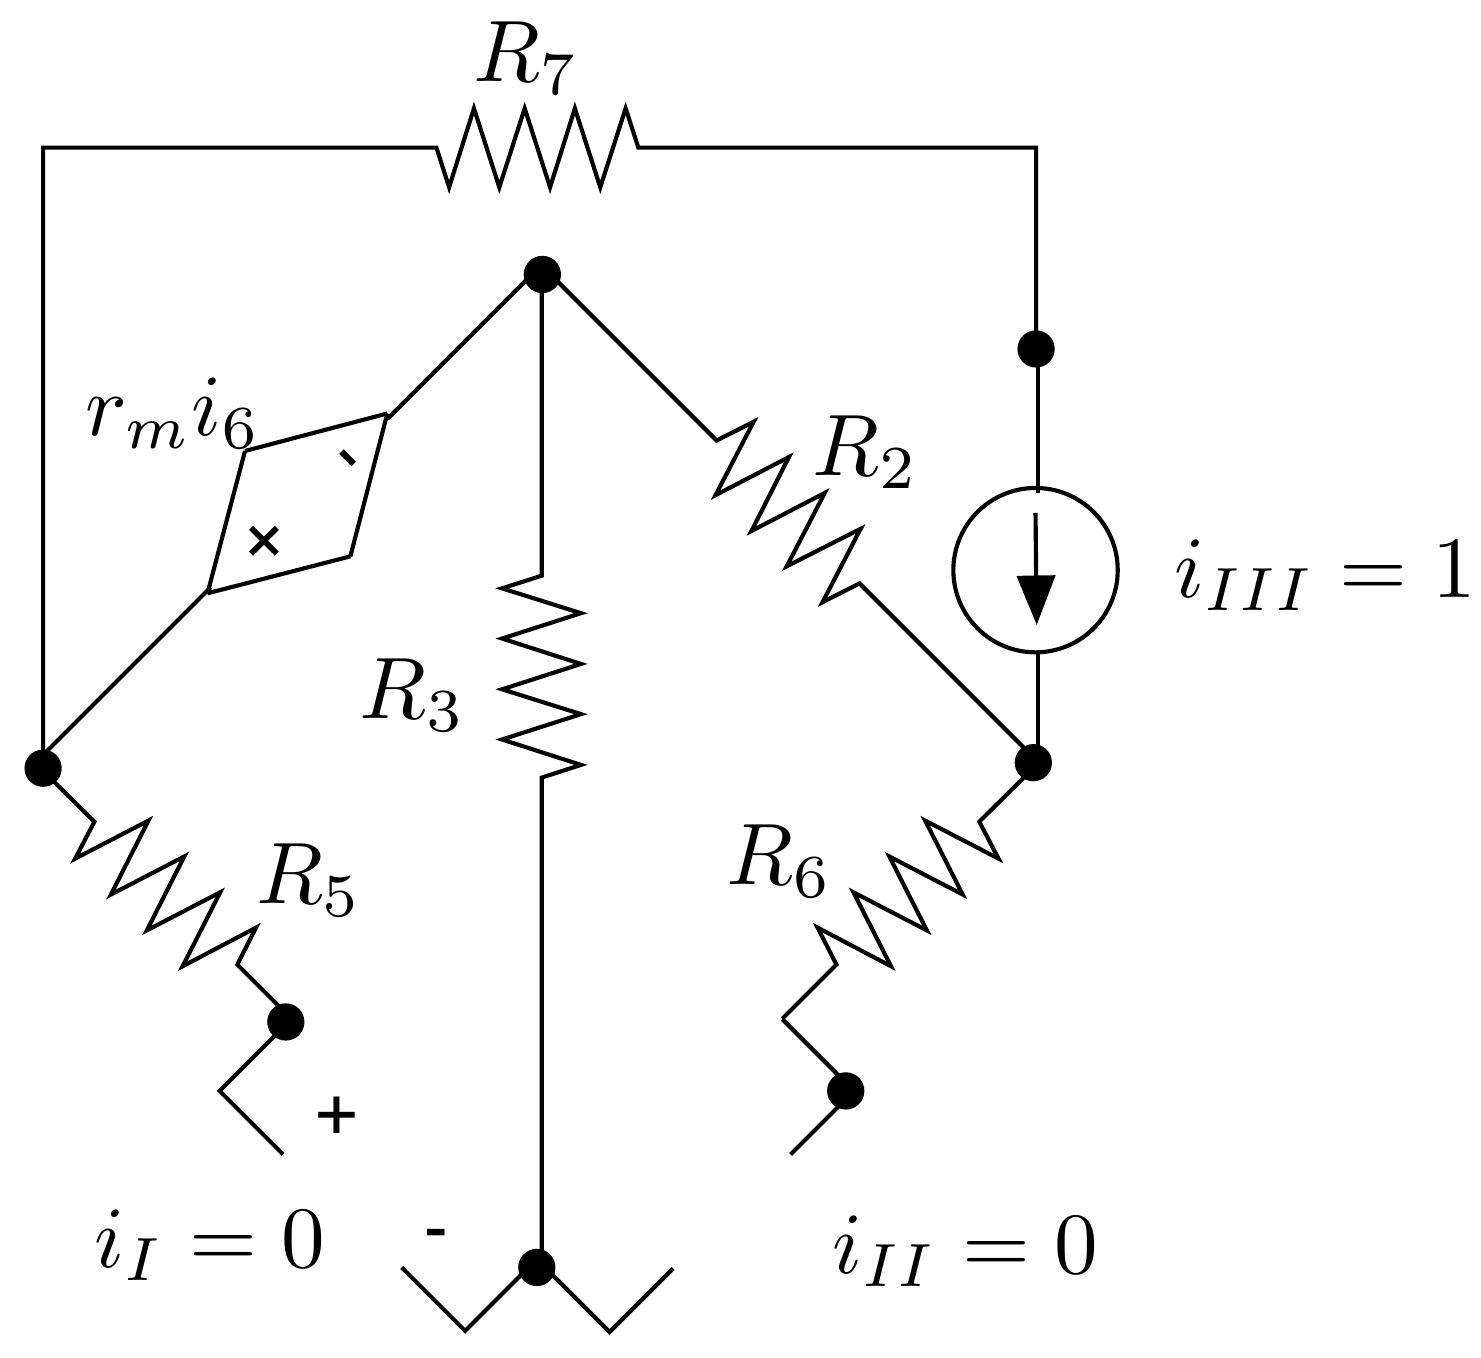
\includegraphics[max width=\textwidth, alt={}]{cbd435a9-cec2-4dd4-b13c-7b225dcc6548-34_1358_1481_448_616}
\end{center}

$$
\begin{gathered}
i_{6}=0 \\
R_{13}=v_{I}=0
\end{gathered}
$$

Exercice : appliquer la méthode expérimentale pour déterminer les éléments de la matrice $\mathbf{R}_{M}$ et en déduire la règle de calcul par inspection.

\section*{Et si le circuit comporte des sources indépendantes de courant}
\begin{itemize}
  \item source en parallèle avec une résistance : transformer la source de courant en une source de tension équivalente
  \item source seule dans une branche : transformer le circuit de la manière suivante\\
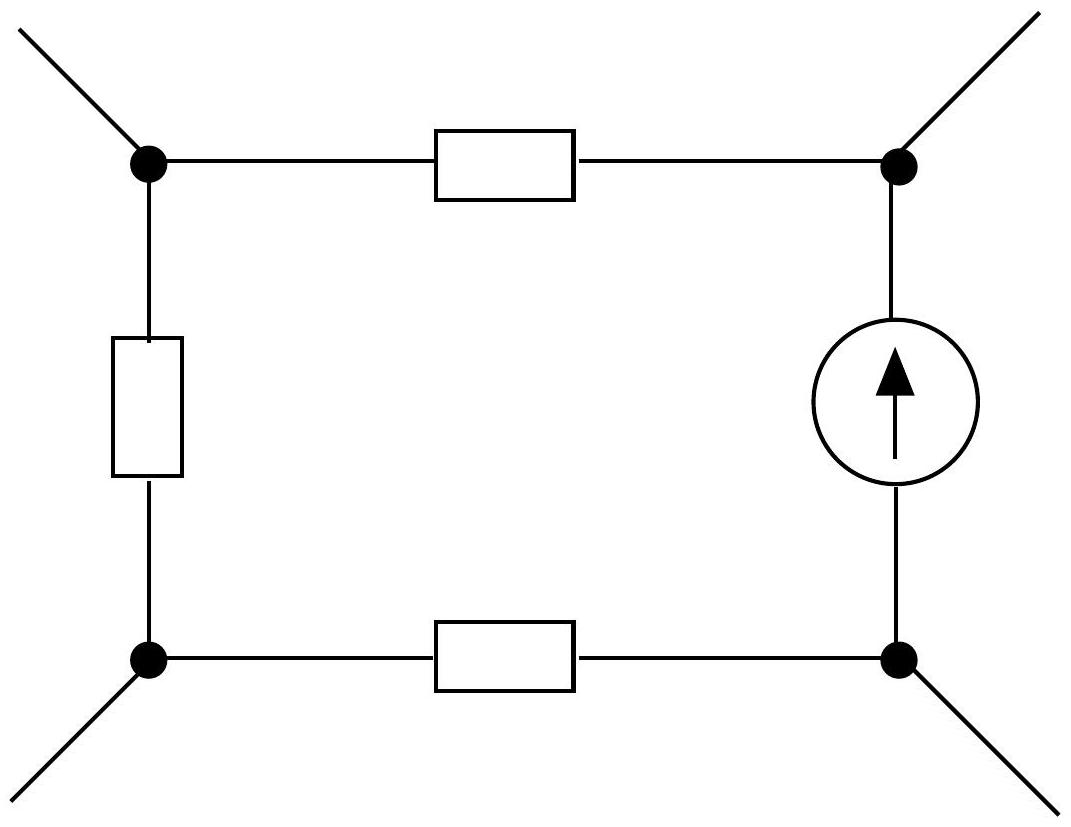
\includegraphics[max width=\textwidth, alt={}, center]{cbd435a9-cec2-4dd4-b13c-7b225dcc6548-35_827_1071_1022_372}\\
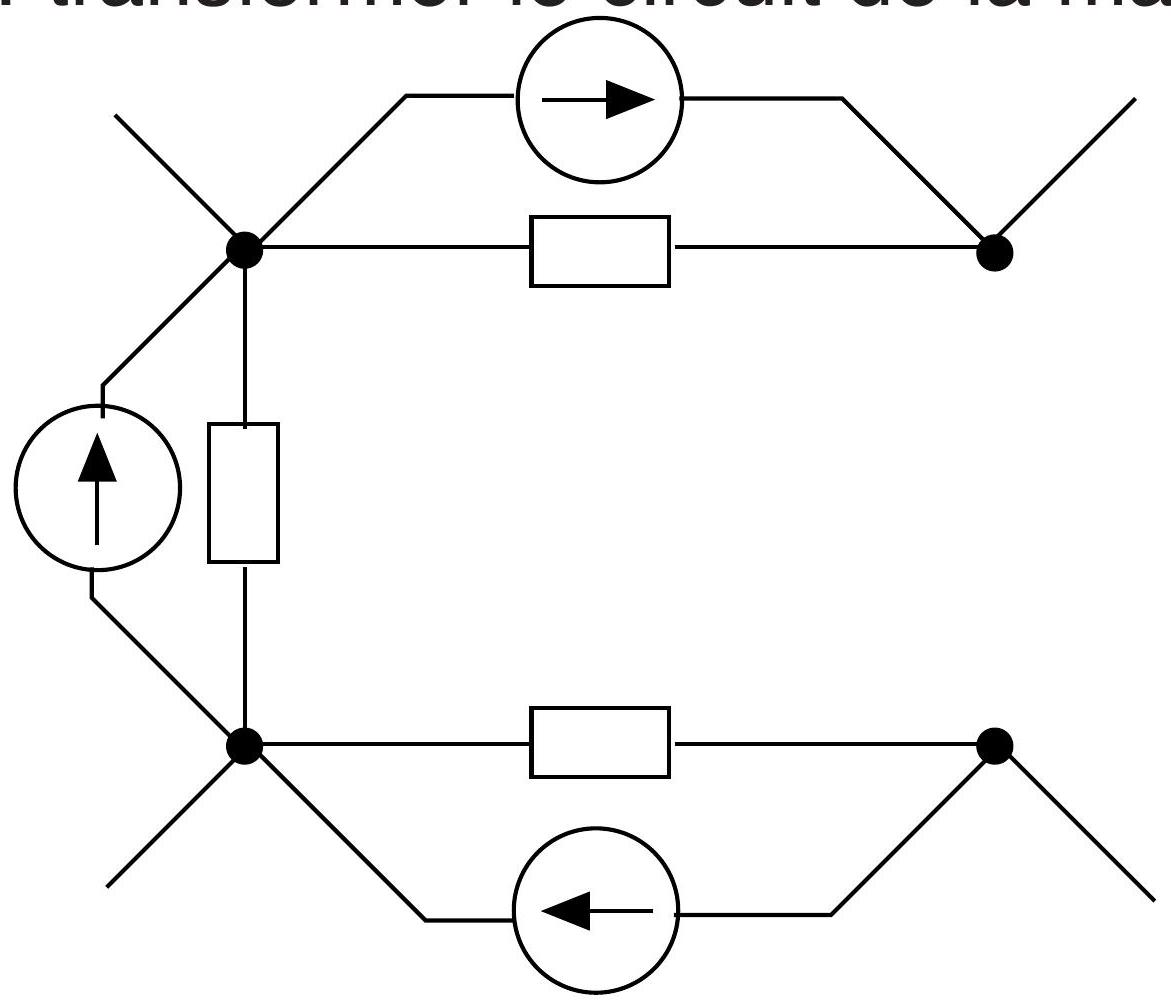
\includegraphics[max width=\textwidth, alt={}, center]{cbd435a9-cec2-4dd4-b13c-7b225dcc6548-35_1003_1171_936_1604}
\end{itemize}

On vérifie que dans le reste du circuit, les LK sont inchangées.\\
!! La branche dans laquelle se trouve la source ne doit pas être couplée avec le reste du circuit (par une source commandée par exemple)

\section*{Théorème de Thévenin généralisé à plusieurs accès}
Partir du schéma équivalent du circuit déduit de la méthode des mailles. Considérer $M=b-(n-1)$ accès, on ouvre chaque maillon pour y placer un accès.\\
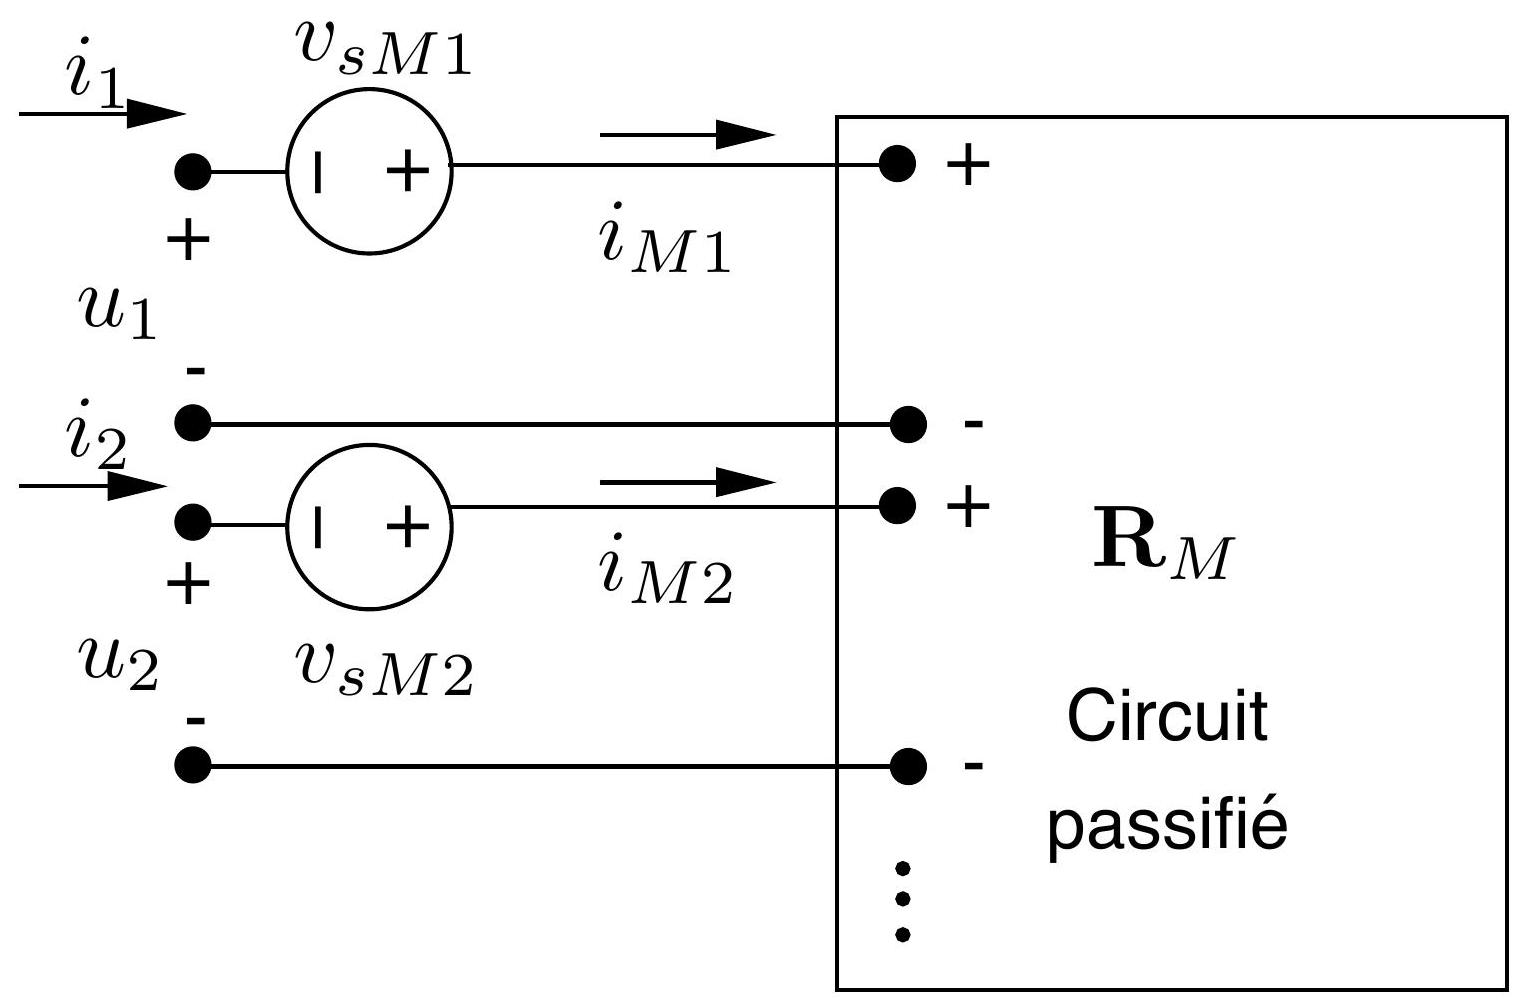
\includegraphics[max width=\textwidth, alt={}, center]{cbd435a9-cec2-4dd4-b13c-7b225dcc6548-36_1003_1526_843_209}

Relations $u-i$ pour les $M$ accès:

$$
\begin{aligned}
\mathbf{u} & =-\mathbf{v}_{s M}+\mathbf{R}_{M} \mathbf{i}_{M} \\
\mathbf{u} & =-\mathbf{v}_{s M}+\mathbf{R}_{M} \mathbf{i}
\end{aligned}
$$

= Schéma équivalent de Thévenin à $M$ accès :

$$
\mathbf{v}_{T h}=-\mathbf{v}_{s M}, \quad \mathbf{R}_{T h}=\mathbf{R}_{M}
$$

\section*{Exemple}
\begin{center}
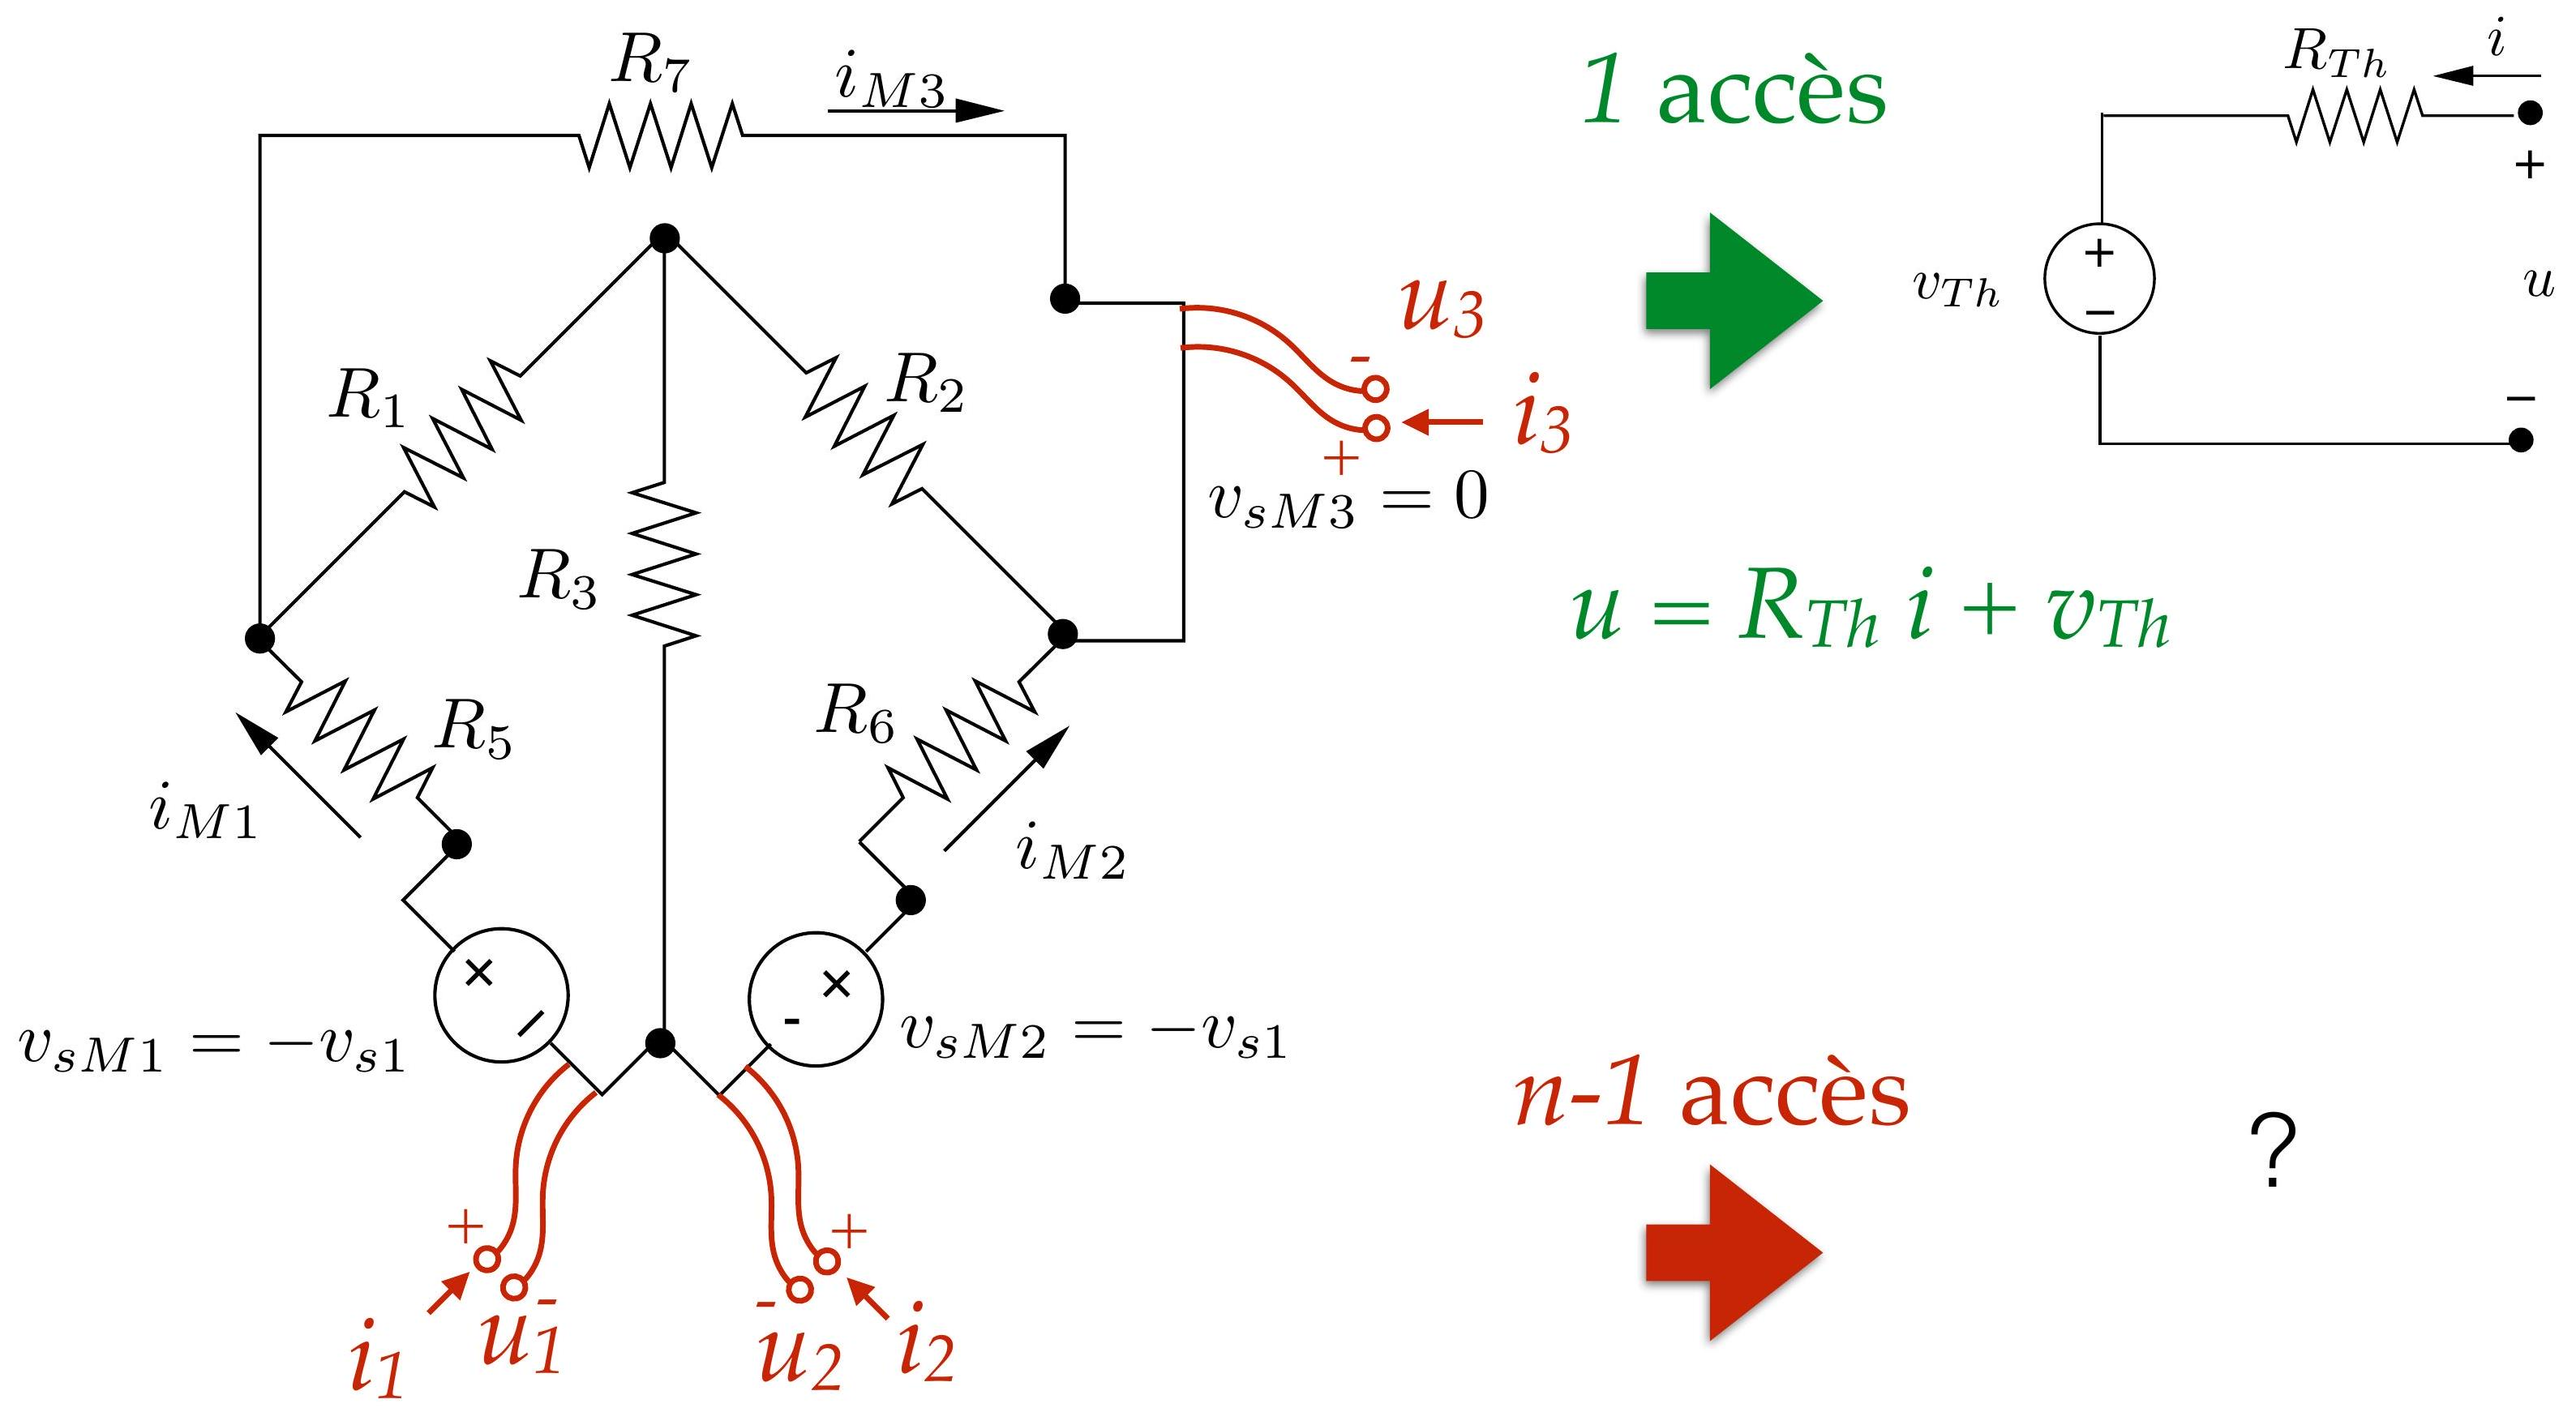
\includegraphics[max width=\textwidth, alt={}]{cbd435a9-cec2-4dd4-b13c-7b225dcc6548-37_1758_3177_463_23}
\end{center}

Soit $a$ le nombre d'accès intéressants (a) (desquels on observe le circuit). Les accès inintéressants sont court-circuités de manière à préserver la topologie du circuit. (b)

$$
u_{a+1}, \ldots, u_{M}=0
$$

\begin{center}
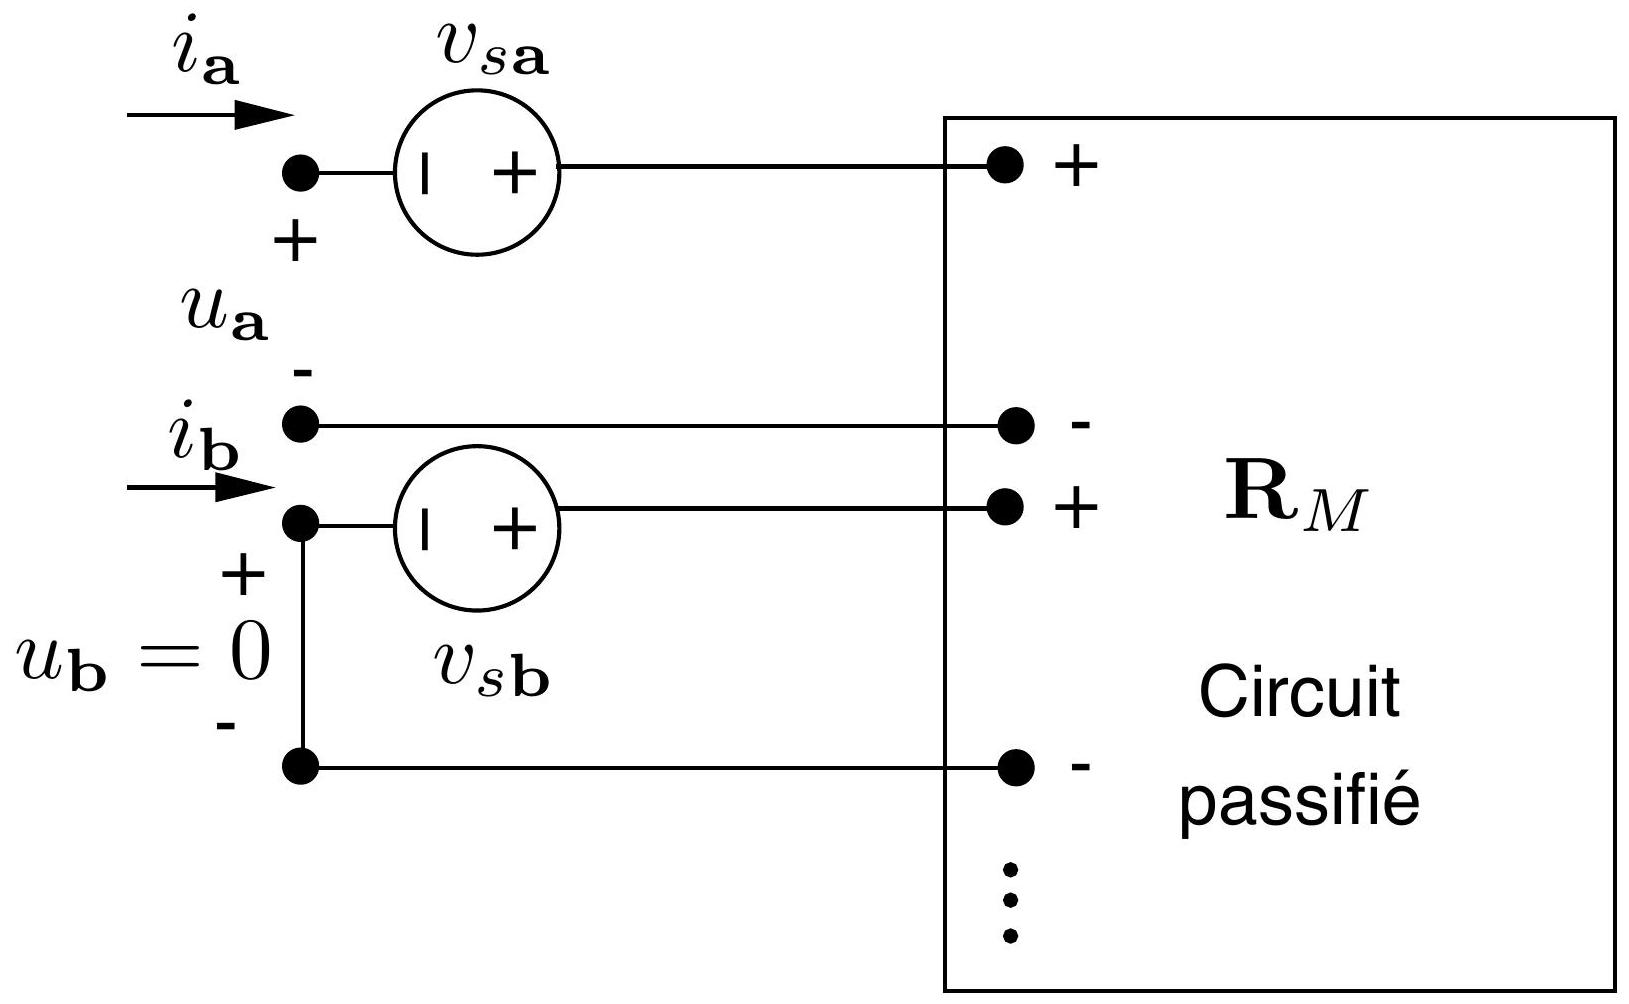
\includegraphics[max width=\textwidth, alt={}]{cbd435a9-cec2-4dd4-b13c-7b225dcc6548-38_1004_1629_1002_907}
\end{center}

On partitionne les relations $u-i$ de la méthode des mailles comme suit :

$$
\begin{gathered}
{\left[\begin{array}{c}
\mathbf{u}_{\mathbf{a}} \\
\mathbf{u}_{\mathbf{b}}
\end{array}\right]=-\left[\begin{array}{c}
\mathbf{v}_{s \mathbf{a}} \\
\mathbf{v}_{s \mathbf{b}}
\end{array}\right]+\left[\begin{array}{ll}
\mathbf{R}_{\mathbf{a}, \mathbf{a}} & \mathbf{R}_{\mathbf{a}, \mathbf{b}} \\
\mathbf{R}_{\mathbf{b}, \mathbf{a}} & \mathbf{R}_{\mathbf{b}, \mathbf{b}}
\end{array}\right]\left[\begin{array}{c}
\mathbf{i}_{\mathbf{a}} \\
\mathbf{i}_{\mathbf{b}}
\end{array}\right]} \\
\mathbf{u}_{\mathbf{b}}=0=-\mathbf{v}_{s \mathbf{b}}+\mathbf{R}_{\mathbf{b}, \mathbf{a}} \mathbf{i}_{\mathbf{a}}+\mathbf{R}_{\mathbf{b}, \mathbf{b}} \mathbf{i}_{\mathbf{b}} \rightarrow \mathbf{i}_{\mathbf{b}}=\mathbf{R}_{\mathbf{b}, \mathbf{b}}^{-1}\left(\mathbf{v}_{s \mathbf{b}}-\mathbf{R}_{\mathbf{b}, \mathbf{a}} \mathbf{i}_{\mathbf{a}}\right) \\
\mathbf{u}_{\mathbf{a}}=\left(-\mathbf{v}_{s \mathbf{a}}+\mathbf{R}_{\mathbf{a}, \mathbf{b}} \mathbf{R}_{\mathbf{b}, \mathbf{b}}^{-1} \mathbf{v}_{s \mathbf{b}}\right)+\left(\mathbf{R}_{\mathbf{a}, \mathbf{a}}-\mathbf{R}_{\mathbf{a}, \mathbf{b}} \mathbf{R}_{\mathbf{b}, \mathbf{b}}^{-1} \mathbf{R}_{\mathbf{b}, \mathbf{a}}\right) \mathbf{i}_{\mathbf{a}}
\end{gathered}
$$

Finalement :

$$
\mathbf{u}_{\mathbf{a}}=\mathbf{v}_{T h}+\mathbf{R}_{T h} \mathbf{i}_{\mathbf{a}}
$$

\section*{Paramètres du schéma équivalent}
Vecteur des sources équivalentes de Thévenin :

$$
\mathbf{v}_{T h}=-\mathbf{v}_{s \mathbf{a}}+\mathbf{R}_{\mathbf{a}, \mathbf{b}} \mathbf{R}_{\mathbf{b}, \mathbf{b}}^{-1} \mathbf{v}_{s \mathbf{b}}
$$

$=$ vecteur des tensions aux bornes des accès à vide ( $\mathbf{i}_{\mathbf{a}}=\mathbf{0}$ )\\
Matrice de résistances de Thévenin = matrice de résistances "réduite" aux accès :

$$
\mathbf{R}_{T h}=\mathbf{R}_{\mathbf{a}, \mathbf{a}}-\mathbf{R}_{\mathbf{a}, \mathbf{b}} \mathbf{R}_{\mathbf{b}, \mathbf{b}}^{-1} \mathbf{R}_{\mathbf{b}, \mathbf{a}}
$$

Peut être déterminée par expérimentation mais jamais par inspection


\end{document}